\documentclass[11pt,twoside]{book}

%\usepackage[draft]{djb}
\usepackage{shortcuts}
\usepackage{fullpage}
\usepackage{fancyhdr}
\pagestyle{fancyplain}
\usepackage{code}
\usepackage{subfig}
\usepackage{listings}
\usepackage{url}
\usepackage{verbatim}
\usepackage{graphicx}
\usepackage{placeins}
\usepackage{xspace}
\usepackage{amsfonts,amsmath,amssymb,amsthm}
\usepackage{hyperref}
\usepackage{proof}
\usepackage{cite}

\newcommand{\doctitle}{The \bap Handbook}
\pagestyle{fancy}

\newcommand{\cmdline}[1]{\texttt{#1}}

%\lhead[\fancyplain{}{\bfseries \thepage}]%
%      {\fancyplain{}{\bfseries\doctitle}}
%\chead[]{}
%\rhead[\fancyplain{}{\bfseries\doctitle}]%
%      {\fancyplain{}{\bfseries \thepage}}
%\lfoot[{\small\scshape Lecture Notes}]{{\small\scshape Lecture Notes}}
%\cfoot[]{}
%\rfoot[{\small\scshape\date}]{{\small\scshape\date}}

\begin{document}

\title{\doctitle}
\author{David Brumley, Ivan Jager, Edward J. Schwartz, and Spencer Whitman}
\date{\today}

\maketitle
\thispagestyle{plain}

\frontmatter

%\input{abstract}
\tableofcontents
\listoffigures
\listoftables

\mainmatter

%\maketitle

\chapter{Introduction}
\section{The Need for Binary Analysis}
\label{vine:introduction}

% We would like to develop software security solutions that are widely
% applicable and offer strong guarantees. 

% We take a binary-centric approach to software security because binary
% code is everywhere, and binary code is faithful to what will actually
% be executed on hardware. Effective security-centric binary analysis
% techniques can potentially impact a wide audience, and provide strong
% guarantees as to what will actually be executed.

Binary code is everywhere. In most situations, users only have access
to code in binary (i.e., executable) form.  Most common, off-the-shelf
(COTS) software (e.g., Microsoft Windows, Adobe Acrobat, etc.) is only
available to end-users in binary form.  Malicious code (i.e., malware)
created by attackers is typically only available in binary form.  The
ubiquity of binary code ensures that security techniques which only
require access to the program binary are likely to be widely
applicable. Further, binary code analysis allows us to argue about the
security of the code that will run, not just the code that was
compiled.


A binary-centric approach to software security requires the ability to
perform program analysis on binary code. A program analysis (whether
it be static or dynamic) is an algorithm for determining the effects
of a set of statements in the programming language under
consideration.  Thus, a binary-centric approach requires 1) the
ability to analyze each instruction in a manner faithful to its
semantics, and 2) a method for encoding an algorithm over those
instructions.

However, there are two primary challenges to performing accurate and
faithful analysis on modern binary code. First, code analysis at the
binary level is different than source code because binary code lacks
many abstractions found in higher-level languages. Second, binary code
is significantly more complex than source code, which introduces new
engineering challenges for binary code analysis.  

% We have developed \emph{\bap}, a \underline{B}inary
% \underline{A}nalysis \underline{P}latform, which addresses these
% challenges. At the heart of \bap is a) a simplified, formally-specific
% intermediate language for assembly, and b) a set of core analysis that
% appropriate for binary code.

\paragraph{Binary Code Analysis is Different than Source Code Analysis.}
Binary code is different than source code. Thus, we must develop and
only use program analyses that are suitable for the unique
characteristics of binary code.  In particular, binary code lacks
abstractions that are often fundamental to source code and source code
analysis, such as:
\begin{itemize}
\item {\bf Functions.} The function abstraction does not exist at the
  binary level.  Instead, control flow in a binary program is
  performed by jumps. For example, the x86 instruction {\tt call x} is
  just syntactic sugar (i.e., shorthand) for storing the number in the
  instruction pointer register {\tt eip} at the address named by the
  register {\tt esp}, decrementing {\tt esp} by the architecture word
  size, and then loading the {\tt eip} with number {\tt x}. Indeed, it
  is perfectly valid in assembly, and sometimes happens in practice,
  that one may call into the middle of a ``function'', or have a
  single ``function'' separated into non-contiguous pieces. The lack
  of a function abstraction poses significant scalability challenges
  to binary analysis.

\item {\bf Memory vs. Buffers.} Binary code does not have buffers, it
  has \emph{memory}.  While the OS may determine a particular memory
  page is not valid, memory does not have the traditional semantics of
  a user-specified type and size. One implication of the difference
  between buffers and memory is that in binary code there is no such
  thing as a buffer overflow. While we may say a particular store
  violates a higher-level semantics given by the source code, such
  facts are inferences with respect to the higher-level semantics, not
  part of the binary code itself. The lack of buffers means we have to
  conservatively reason about the entire memory space (unless proven
  otherwise) at each operation.

\item {\bf No Types.} New types cannot be created or used since there
  is no such thing as a type constructor in binary code. The only
  types available are those provided by the hardware: registers and
  memory.  Even register types are not necessarily a good choice,
  since it is common to store values from one register type (e.g.,
  32-bit register) and read them as another (e.g., 8-bit
  register). The lack of types means we cannot use type-based
  analysis, which is often instrumental in scaling traditional
  analyses.

\end{itemize}


\paragraph{Binary Code is Complex.}

\begin{figure}
\begin{minipage}{.4\linewidth}
\begin{code}
// instr dst,src
1. add eax, ebx
2. shl eax, edx
3. jo target
4. ....
...
target: ...
\end{code}
\end{minipage}
\begin{minipage}[c]{.5\linewidth}
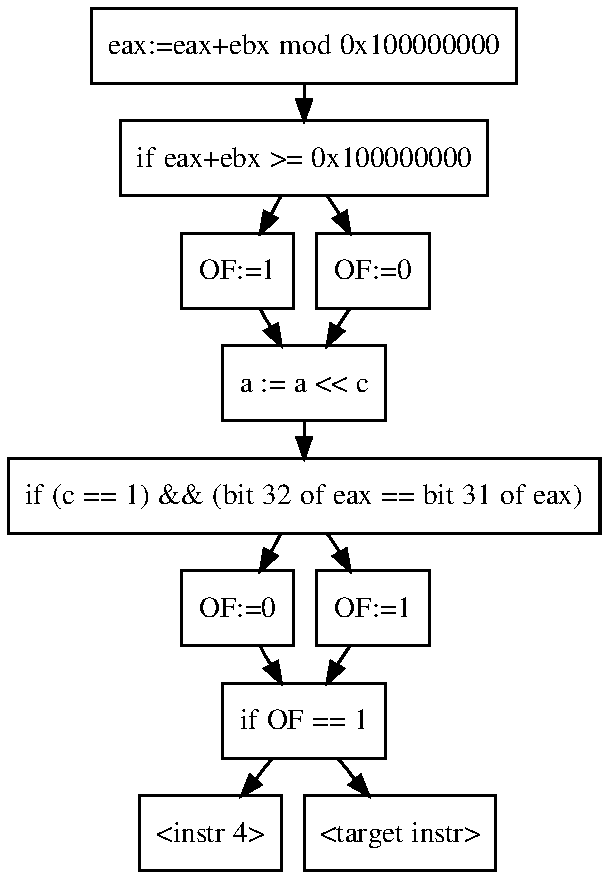
\includegraphics[scale=.5]{fig/add-shl}
\end{minipage}
\caption{A three instruction x86 program, and its corresponding
  control flow graph.  Note the logic for deciding when the jump on
  overflow instruction (statement 3) is taken, when is often omitted
  by other binary analysis platforms. }
\label{vine:shl-add}
\end{figure}

One approach is to disassemble binary code into a sequence of assembly
instructions, and then perform program analysis directly over the
assembly instructions.  This type of assembly-specific approach is
\naive because each analysis would have to individually understand the
semantics of the assembly, which is difficult.

For example, consider the basic program analysis problem of
determining when the conditional jump is taken on line 3 of
Figure~\ref{vine:shl-add}. In this example, all operands are 32-bit
registers, and all arithmetic is therefore performed mod
$2^{32}$. Instruction 1 computes the sum {\tt eax := eax+ebx} (mod
$2^{32}$).  Instruction 2 computes {\tt eax = eax $\ll$ edx}.  Both
instructions may set the overflow status register {\tt OF}. The {\tt
  add} instruction will set the {\tt OF} flag if {\tt eax + ebx $\geq$
  $2^{32}$}.  The {\tt shl} instruction will set the {\tt OF} flag if
{\tt edx} is 1 \emph{and} the top two bits of {\tt eax} are not equal
on line 2. The instruction on line 3 tests to see if {\tt OF} is set,
and if so, jumps to {\tt target}, else executes the next sequential
instruction. 

In order to determine when the jump on line 3 is taken, an analysis
must reconstruct all side-effects of {\tt add} and {\tt shl}.  The
proper control flow diagram is shown in Figure~\ref{vine:shl-add}.  As
demonstrated by this three line program, even though a program may
look simple, determining the effects may be complicated. An
assembly-specific approach would require each analysis to reason about
such complex semantics.


Worse, many architectures allow instruction prefixes, which can
further complicate the semantics. For example, in x86 a {\tt rep}
prefix essentially turns an instruction into a single instruction
loop, e.g., {\tt rep $i$ $s$,$d$} will repeatedly execute operation
$i$ on arguments $s$ and $d$.  The exact semantics (per
Intel~\cite{intel:x86}) of {\tt rep} are shown in
Figure~\ref{vine:rep}. An assembly-specific approach would have to
consider this complicated logic for any instruction that may carry the
{\tt rep} prefix. If analyses are written directly on assembly, each
analysis would duplicate this logic.


\begin{figure}
\begin{footnotesize}
\begin{code}
  IF AddressSize = 16 
  THEN 
     Use CX for CountReg; 
  ELSE IF AddressSize = 64 and REX.W used 
     THEN Use RCX for CountReg; FI; 
  ELSE 
     Use ECX for CountReg; 
  FI; 
  WHILE CountReg $\neq$ 0 
  DO 
      Service pending interrupts (if any); 
      Execute associated string instruction ($x$);  
      CountReg $\leftarrow$ (CountReg – 1); 
      IF CountReg = 0 
      THEN exit WHILE loop; FI; 
      IF (Repeat prefix is REPZ or REPE) and (ZF = 0) 
         or (Repeat prefix is REPNZ or REPNE) and (ZF = 1) 
      THEN exit WHILE loop; FI; 
  OD; 
\end{code}
\end{footnotesize}
\caption{The semantics of the {\tt rep} instruction according to
  Intel~\cite{intel:x86}. Modern architectures often have hundreds of
  instructions that have complex semantics like {\tt rep}.}
\label{vine:rep}
\end{figure}

If there were only a few instructions, perhaps the complexity would
not be too onerous.  Modern architectures, however, typically have
hundreds of instructions. x86, for example, has well over 300
instructions (which are documented in over 11 lbs of
manuals~\cite{intel:x86}).

% This is very outdated now.
% Overall, an assembly specific approach is unattractive because writing
% analyses over modern instruction sets tends to be tedious and
% error-prone. For example, the current version of
% DynInst~\cite{dyninst} (version 5.2) and Phoenix~\cite{phoenix} (April
% 2008 SDK Build), two popular architectures for binary analysis, will
% not create a correct control flow graph for the three line program.
% Verifying a program analysis is correct over a large and complicated
% instruction set seems even more difficult.
% Further, an
% assembly-specific approach is specific to a single architecture.  All
% analysis would have to be ported each time we want to consider a new
% architecture.  Thus, analysis could not take advantage of the common
% semantics across many different assemblies.


\section{Desired Properties}

We would like a platform for analyzing binary code that 1) supports
writing analyses in a concise and straight-forward fashion, 2)
provides abstractions for common semantics across all assemblies, and
3) is architecture independent when possible.

We want an architecture that supports writing analyses in a concise,
straight-forward fashion because that makes it easier to write
analyses that are correct.  We do not want an analysis to have to
tangle with complicated instruction semantics: that should be the
job of the architecture.  
%Simplifying analysis is challenging,
%however, because modern architectures are designed for computational
%efficiency, not ease of understanding.

We would also like to provide abstractions that are common to typical
program analyses. There are many recurring abstractions. One is to be
able to iterate over each instruction type. Another is to build a
control flow graph.  Yet another is finding data dependencies. We
would like to build a single platform so that a new program analysis
can easily reuse common abstractions.

Finally, we would like to be architecture independent.  Architecture
independence would allow us to easily re-target the entire platform to
a new architecture without changing the analyses.  The more
architectures we can handle, the more widely our techniques will be
applicable.



% modern instructions is likely at best to difficult to create,
% difficult to debug, and difficult to show correct.




% . One reason is an
% assembly-specific approach is specific to only the single assembly for
% the architecture under consideration. Second, writing program analysis
% over assembly directly is tedious and error-prone.  Modern
% architectures such as x86 typically have hundreds of instructions,
% each of which may have complex semantics.  As a result, a typical
% program analysis may have to consider hundreds of cases, and each case
% may be associated with extensive code to handle the complexity of a
% particular instruction.

%%% Local Variables: 
%%% mode: latex
%%% TeX-master: "../main"
%%% End: 

\section{\bap Overview}

\begin{figure}
\centering
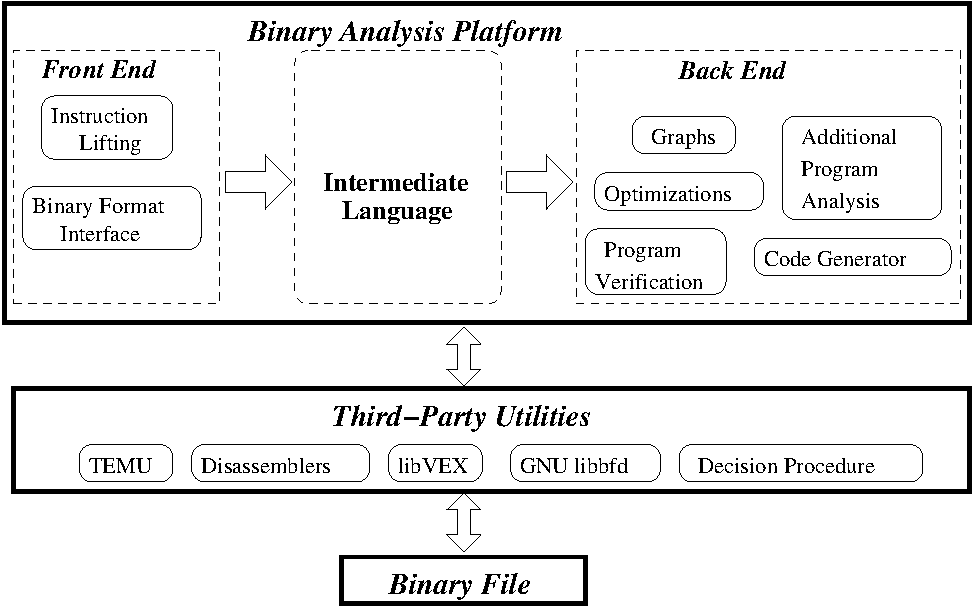
\includegraphics[scale=.8]{fig/components}
\caption{The \bap binary analysis architecture and components. \bap
  is divided into a front-end, which is responsible for lifting
  instructions to the \bap IL, and a platform-independent back-end
  for analyses.}
\label{fig:vine-components}
\end{figure}

\bap  is designed to facilitate faithful
security-relevant binary program analysis by 1) reducing complex
instruction sets to a single, small, and formally specified
intermediate language that supports writing  concise,
easy-to-understand analyses 2) providing a set of core program analyses
abstractions, and 3) being architecture independent when possible in
order to support easy re-targeting.


Figure~\ref{fig:vine-components} shows a high-level picture of \bap.
\bap is divided into an architecture-specific front-end and an
architecture-independent back-end.  At the core of \bap is an
architecture-independent intermediate language (IL), called \emph{\bil,} for
assembly. Assembly instructions in the underlying architecture are
lifted up to the \bil via the \bap front-end.  All analyses are
performed on the platform-independent \bil in the back-end.
%Thus, program analysis can be
%written in an architecture-independent fashion.

We lift to the \bil by using open-source utilities to parse the binary
format and produce assembly.  The assembly is then lifted up to the
\bap IL in a syntax-directed manner. The \bap front-end currently
supports lifting usermode x86~\cite{intel:x86} code, though other
architectures may be added to the \bap framework.
% and ARMv4~\cite{arm:armv4} to the IL.

The \bap back-end supports a variety of core program analyses
and utilities.  The back-end has utilities for creating a variety of
different graphs, such as control flow and program dependence graphs.
The back-end also provides an optimization framework. The optimization
framework is usually used to simplify a specific set of
instructions. We also provide program verification capabilities such
as symbolic execution, calculating the weakest precondition, and
interfacing with decision procedures.  \bap can also write out lifted
\bap instructions as valid C code via the code generator back-end.

%%% Local Variables: 
%%% mode: latex
%%% TeX-master: "../main"
%%% End: 


\chapter{The \bap Toolkit}
\section{\bap Overview}

\begin{figure}
\centering
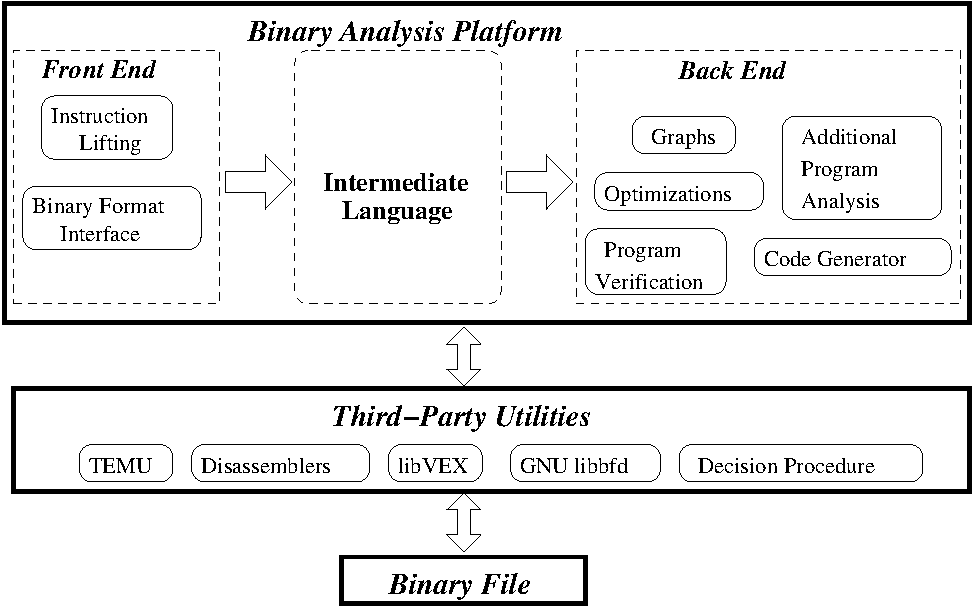
\includegraphics[scale=.8]{fig/components}
\caption{The \bap binary analysis architecture and components. \bap
  is divided into a front-end, which is responsible for lifting
  instructions to the \bap IL, and a platform-independent back-end
  for analyses.}
\label{fig:vine-components}
\end{figure}

\bap  is designed to facilitate faithful
security-relevant binary program analysis by 1) reducing complex
instruction sets to a single, small, and formally specified
intermediate language that supports writing  concise,
easy-to-understand analyses 2) providing a set of core program analyses
abstractions, and 3) being architecture independent when possible in
order to support easy re-targeting.


Figure~\ref{fig:vine-components} shows a high-level picture of \bap.
\bap is divided into an architecture-specific front-end and an
architecture-independent back-end.  At the core of \bap is an
architecture-independent intermediate language (IL), called \emph{\bil,} for
assembly. Assembly instructions in the underlying architecture are
lifted up to the \bil via the \bap front-end.  All analyses are
performed on the platform-independent \bil in the back-end.
%Thus, program analysis can be
%written in an architecture-independent fashion.

We lift to the \bil by using open-source utilities to parse the binary
format and produce assembly.  The assembly is then lifted up to the
\bap IL in a syntax-directed manner. The \bap front-end currently
supports lifting usermode x86~\cite{intel:x86} code, though other
architectures may be added to the \bap framework.
% and ARMv4~\cite{arm:armv4} to the IL.

The \bap back-end supports a variety of core program analyses
and utilities.  The back-end has utilities for creating a variety of
different graphs, such as control flow and program dependence graphs.
The back-end also provides an optimization framework. The optimization
framework is usually used to simplify a specific set of
instructions. We also provide program verification capabilities such
as symbolic execution, calculating the weakest precondition, and
interfacing with decision procedures.  \bap can also write out lifted
\bap instructions as valid C code via the code generator back-end.

%%% Local Variables: 
%%% mode: latex
%%% TeX-master: "../main"
%%% End: 

\section{Obtaining \bap}
Please email David Brumley to get the current \bap URL and credentials.
We currently distribute \bap as a VMWare virtual machine. We
distribute \bap in a virtual machine for several reasons. First, \bap
has quite a few dependencies, thus setup is potentially
complex. Second, while we do not provide support, issues that we
choose to resolve can be done more quickly when we know the exact
setup.



\section{\texttt{toil}: Lifting Binary Code to \bil}

The {\tt toil} tool lifts binary code to \bil.  Lifting up binary code
to the IL consists of two steps:
\begin{itemize}
\item First, the binary file is opened using libbfd. BAP can read
  binaries from any bfd-supported binary, including ELF and PE
  binaries.

\item Second, the executable code in the binary is disassembled.  {\tt
  toil} currently uses a linear sweep disassembler.

\item Each assembly instruction discovered by the linear sweep disassembler
  is then lifted directly to \bil.
\end{itemize}

Lifted assembly instructions have all of the side-effects explicitly
exposed.  As a result, a single typical assembly instruction will be
lifted as a sequence of \bil instructions.  For example, the {\tt add
  \$2, \%eax} instruction is lifted as:

\begin{centering}
\begin{scriptsize}
\begin{verbatim}
addr 0x0 @asm "add    $0x2,%eax"
label pc_0x0
T_t1:u32 = R_EAX:u32
T_t2:u32 = 2:u32
R_EAX:u32 = R_EAX:u32 + T_t2:u32
R_CF:bool = R_EAX:u32 < T_t1:u32
R_OF:bool = high:bool((T_t1:u32 ^ ~T_t2:u32) & (T_t1:u32 ^ R_EAX:u32))
R_AF:bool = 0x10:u32 == (0x10:u32 & (R_EAX:u32 ^ T_t1:u32 ^ T_t2:u32))
R_PF:bool =
  ~low:bool(R_EAX:u32 >> 7:u32 ^ R_EAX:u32 >> 6:u32 ^ R_EAX:u32 >> 5:u32 ^
            R_EAX:u32 >> 4:u32 ^ R_EAX:u32 >> 3:u32 ^ R_EAX:u32 >> 2:u32 ^
            R_EAX:u32 >> 1:u32 ^ R_EAX:u32)
R_SF:bool = high:bool(R_EAX:u32)
R_ZF:bool = 0:u32 == R_EAX:u32
\end{verbatim}
\end{scriptsize}
\end{centering}

The lifted \bil code explicitly detail all the side-effects of the
{\tt add} instruction, including all six flags that are updated by the
operation.  As another example, an instruction with the {\tt rep}
prefix (whose semantics are in Figure~\ref{vine:rep}) is lifted as a
sequence of statements that form a loop.

In addition to binary files, {\tt toil} can also lift an instruction
trace to the IL.  The most recent BAP trace format can be lifted using
the {\tt -trace} option.

{\tt toil} can output to several formats for easy parsing, including
protobuf, JSON, and XML.  These formats are selected via the {\tt
  -topb}, {\tt -tojson}, and {\tt -toxml} options.  Code for reading
the protobuf encoding is in the {\tt piqi-files/protobuf} directory.

%%% Local Variables: 
%%% mode: latex
%%% TeX-master: "../main"
%%% End: 

\section{\texttt{iltrans}: Programs Transformations on \bil Code}
The {\tt iltrans} tool applies transformations and analyses to \bil.
The arguments to {\tt iltrans} specify a sequence of transformations,
optionally printing out the result of the transformation.  For
example, executing:
\begin{verbatim}
 iltrans -trans1 -trans2 outfile -trans3 infile
\end{verbatim}
would read in {\tt infile}, perform transformation {\tt trans1}, the
output of which is fed to {\tt trans2}, the output of which is again
fed to {\tt trans3} as well as printed to {\tt outfile}. Although this
may seem a little strange at first, the tool is designed to make it
easy to specify exactly what algorithms you wish to perform over the
IL.


{\tt iltrans} provides a library of common analyses and utilities,
which can be used as building blocks for more advanced analyses.
Please consult {\tt iltrans -help} for exact arguments.  We detail
below at a high level several of the analysis that can be performed by
{\tt iltrans}


% \paragraph{Type Checker.
% \item {\bf Type checker.}  The \bap IL serves both as an intermediate
%   representation for assembly and as a programming language that
%   assembly-like programs can be written in.  However, the \bap IL
%   syntax from Figure~\ref{vine:syntax} permits several undefined
%   operations.  For example, the syntax allows adding two variables of
%   different types. The \bap type-checker further restricts the
%   language by removing obviously meaningless statements, as well as
%   catching several typical bugs. The \bap type-checking is not
%   designed to ensure safety (preservation + progress) of a
%   type-checked program. Chapter~\ref{vine:typecheck} details \bap
%   type-checking.


\paragraph{Graphs.} {\tt iltrans} provides options for building and
manipulating control flow graphs (CFG), including a pretty-printer for
the graphviz DOT graph language~\cite{graphviz:dot}. {\tt iltrans}
also provides options for building data, control, and program
dependence graphs~\cite{muchnick:1997}.  These graphs can be output in
the {\tt dot} language.  The graphs themselves can be quite large.  We
currently use {\tt zgrviewer}~\cite{zgrviewer} for viewing the
resulting dot files.


One issue when constructing  graphs of an assembly program is
determining the successors of jumps to computed values, called {\it
  indirect} jumps.  Resolving indirect jumps usually involves a program
analysis that require a CFG, e.g., VSA~\cite{balakrishnan:2007}. Thus,
there is a potential circular dependency.  Note that an indirect jump
may potentially go anywhere, including the heap or code that has not
been previously disassembled.

Our solution is to designate a special node as a successor of
unresolved indirect jump targets in the CFG.  We provide this so an
analysis that depends on a correct CFG can recognize that we do not
know the subsequent state. For example, a data-flow analysis could
widen all facts to the lattice bottom.  Most normal analyses will
first run an indirect jump resolution analysis in order to build a
more precise CFG that resolves indirect jumps to a list of possible
jump targets.  %% {\tt iltrans} provides one such analysis, called Value Set
%% Analysis~\cite{balakrishnan:2007}.

\paragraph{Single Static Assignment.} {\tt iltrans} supports
conversion to and from single static assignment (SSA)
form~\cite{muchnick:1997}. SSA form makes writing an analysis easier
because every variable is defined statically only once.  Note we
convert both memory and scalars to SSA form. We convert memories so
that an analysis can syntactically distinguish between memories before
and after a write operation instead of requiring the analysis itself
to maintain similar bookkeeping. For example, in the memory
normalization example in Figure~\ref{vine:normalized}, an analysis can
syntactically distinguish between the memory state before the write on
line 1, the write on line 5, and the read on line 7.

\paragraph{Chopping.}  Given a source and sink node, a program
chop~\cite{jackson:1994} is a graph showing the statements that cause
definitions of the source to affect uses of the sink.  For example,
chopping can be used to restrict subsequent analyses to only a portion
of code relevant to a given source and sink instead of the whole
program. %% We describe our implementation of chopping in more detail
%% in~\ref{algs:chopping}.

\paragraph{Data-flow and Optimizations.} {\tt iltrans} interfaces with
the generic data-flow engine in \bap.  The data-flow engine works on
user-defined lattices, such as those for constant propagation, dead
code elimination, etc.  \bap currently implements
Simpson's global value numbering~\cite{simpson:1996}, (aggressive)
dead-code elimination~\cite{muchnick:1997}, and live-variable
analysis~\cite{muchnick:1997}.

We have also implemented value set
analysis~\cite{balakrishnan:2007}. Value set analysis is a data-flow
analysis that over-approximates the values for each variable at each
program point. Value-set analysis can be used to help resolve indirect
jumps. It can also be used as an alias analysis.  Two memory accesses
are potentially aliased if the intersection of their value sets is
non-empty.


Optimizations are useful for simplifying or speeding up subsequent
analyses. For example, we have found that the time for the decision
procedure STP to return a satisfying answer for a query can be cut in
half by first using program optimization to simplify the
query~\cite{brumley:2008}.

%%% Local Variables: 
%%% mode: latex
%%% TeX-master: "../main"
%%% End: 

\section{{\tt topredicate}: Predicate-based Program Verification}

{\tt topredicate} supports program verification in two ways. First,
{\tt topredicate} can convert the IL into Dijkstra's Guarded Command
Language (GCL), and calculate the weakest precondition with respect to
GCL programs~\cite{dijkstra:1976}. The weakest precondition for a
program with respect to a predicate $q$ is the most general condition
such that any input satisfying the condition is guaranteed to
terminate (normally) in a state satisfying $q$.  Currently we only
support acyclic programs, i.e., we do not support GCL {\tt while}.

{\tt topredicate} also interfaces with decision procedures.  {\tt
  topredicate} can write out expressions (e.g., weakest preconditions)
in CVC Lite syntax~\cite{cvclite}, which is supported by several
decision procedures. In addition, {\tt topredicate} interfaces
directly with the STP~\cite{ganesh:2007} decision procedure through
calls from \bap to the STP library.

\section{{\tt ileval}: Concrete evaluation} 

{\tt ileval} evaluates a given \bil
program using the operational semantics in in~\ref{vine:operational}.
The evaluator allows us to execute programs without recompiling the IL
back down to assembly. For example, we can test that a raised program
is correct by executing the IL on an input $i$, observing the value $v$,
executing the original binary program on $i$, observing the value
$v'$, and verifying $v = v'$.

\section{\texttt{codegen}: LLVM-based code generation}

\texttt{codegen} converts a \bil program to LLVM~\cite{llvm} IL, and
then converted to native code using LLVM's code generators.  This may
be useful for translating binary code to other architectures, or for
static instrumentation.

%% We don't have a separate toc command anymore

%% \section{{\tt toc}} 

%% {\tt toc} generates valid C code from the IL.  For example, one could
%% use this as a rudimentary decompiler by first raising assembly to
%% \bil, then writing it out as valid C.  The ability to export to C also
%% provides a way to compile \bil programs: the IL is written as C, then
%% compiled with a C compiler.

%% The C code generator implements memories in the IL as arrays.  A {\tt
%%   store} operation is a store on the array, and a {\tt load} is a load
%% from the array.  Thus, C-generated code simulates real memory.  For
%% example, consider a program that is vulnerable to a buffer overflow
%% attack. It is raised to \bil, then written as C and recompiled. An
%% out-of-bound write on the original program will be simulated in the
%% corresponding C array, but will not lead to a real buffer overflow.


\section{Discussion}
\label{vine:discussion}

\subsection{Why Design a New Infrastructure?}  

At a high level, we designed \bap as a new platform because existing
platforms are a) defined for higher-level languages and thus not
appropriate for binary code analysis, b) designed for orthogonal goals
such as binary instrumentation or decompilation, and/or c) unavailable
to use for research purposes.  As a result, other tools we tried
(e.g., DynInst~\cite{dyninst} version 5.2, Phoenix~\cite{phoenix}
April 2008 SDK, IDA Pro~\cite{idapro} version 5, and others) were
inadequate, e.g., could not create a correct control flow graph for
the 3 line assembly shown in Figure~\ref{vine:shl-add}. Another reason
we created \bap is so that we could be sure of the semantics of 
analysis. Existing platforms tend not to have publicly available
formally defined semantics, thus we would not know exactly what we are
using.

Formal semantics are important for several practical reasons. We found
that defining the semantics of \bap was helpful in catching design
bugs, unsupported assumptions, and other errors that could affect many
different kinds of analysis. In addition, the semantics are helpful
for communicating how \bap works with other researchers.  Further,
without a specified semantics, it is difficult to show an analysis is
correct. For example, in ~\cite{brumley:2006:alias} we show our
proposed assembly-level alias analysis~\cite{brumley:2006:alias} is
correct with respect to the operational semantics of \bap.


\subsection{Limitations of \bap}

\begin{description}
\item[Architectures] \bap only supports x86 right now.  We intend to
  add support for x86-64 and ARM in the future.
\item[Semantics] \bap is designed to enable program analysis of binary
  program states. Therefore, analyses that depend upon more than the
  operational semantics of the instruction fall outside the scope of
  \bap. For example, creating an analysis of the timing behavior of
  binary programs falls outside the current scope of \bap.
\item[User-mode instructions] \bap only models user-mode level
  instructions.  Unhandled instructions will be lifted as {\tt
    special} statements or {\tt unknown} expressions.
\item[Integer instructions] \bap only models instructions that
  manipulate integers.  In particular, \bap does not model floating
  point instructions.
\item[Indirect jumps] \bap does not currently resolve indirect jumps,
  or perform ``CFG recovery''.  We plan to add this in a future
  release.
\end{description}

\subsection{Is Lifting Correct?}

Assembly instructions are lifted to \bap in a syntax directed manner.
One may view the \bap IL as a model of the underlying assembly.  There
is a chance, however, that lifting could produce incorrect
IL. Although it is impossible to say that all assembly instructions
are correctly lifted, the advantage of \bap's design is that only the
lifting process needs to understand the semantics of the original
assembly.

We perform nightly testing to make sure that \bap's model of execution
matches what happens on a real x86 processor.  Our nightly tests also
tell us which instructions are used in our test programs that are not
modeled in \bap.  The results of these tests are always available at
\url{http://bap.ece.cmu.edu/nightly-reports/}.

\subsection{Size of Lifting IL for a Program}

A single assembly instruction will typically be translated into
several \bap statements. Thus, the resulting \bap program will have
more statements than the corresponding assembly.  For example and
roughly speaking, x86 assembly instructions are raised to be about 7
\bap statements: 1 \bap statement for the direct effect, and 6 for
updating processor-specific status flags.

In our experience, the constant-size factor in code size is worth the
benefits of simplifying the semantics of assembly.  Assembly
instructions are designed to be efficient for a computer to execute,
not for a human to understand. The IL, on the other hand, is designed
to be easy for a human to understand.  We have found even experienced
assembly-level programmers will comment that they have a hard time
keeping track of control and data dependencies since there are few
syntactic cues in assembly to help. \bap, on the other hand, obviates
all data and control dependencies within the code. 

%%% Local Variables: 
%%% mode: latex
%%% TeX-master: "../main"
%%% End: 

%\input{chap-tools/translate}


\chapter{Formalization of \bil}

At the core of \bap is the \bap intermediate language, called \bil. In
this chapter we present a formalization of \bil. The formalization is
intended to provide an exact description of what we mean by statements
in the IL.

{\it Note:} In our implementation, as discussed elsewhere, there are
actually several IL's.  Throughout this chapter we discuss the IL as
implemented in {\tt ast.ml}.  The other IL's differ in uninteresting
ways and are variants of the IL discussed here. In particular,
developers will be interested in {\tt ssa.ml}, which defines the IL in
SSA form, and also does not allow recursively defined expressions
(i.e., it is an SSA three-address code).  Thus, this chapter can be
viewed as a specification for the actual code.



\section{The \bil Language}
\label{vine:language}


\begin{table}
\centerbox{
\begin{tabular}{lll}
  \emphkind{program}&::=&
        \emphkind{stmt}*\\

  \emphkind{stmt}&::=&  
         \emphkind{var} := \emphkind{exp}
     $|$ {\tt jmp}(\emphkind{exp})
     $|$ {\tt cjmp}(\emphkind{exp},\emphkind{exp},\emphkind{exp})\\
     &&$|$ {\tt halt}(\emphkind{exp})
     $|$ {\tt assert}(\emphkind{exp})
     $|$ {\tt label} \emphkind{label\_kind}
     $|$ {\tt special}(string)\\

  \emphkind{exp}&::=& 
         {\tt load}(\emphkind{exp}, \emphkind{exp}, \emphkind{exp},
         \emphkind{$\tau_{\text{reg}}$})
        $|$ {\tt store}(\emphkind{exp}, \emphkind{exp},
        \emphkind{exp},\emphkind{exp},$\tau_{\text{reg}}$ )
     $|$ \emphkind{exp} $\Diamond_b$ \emphkind{exp}
     \\
     & & 
     $|$ $\Diamond_u$ \emphkind{exp}
     $|$ \emphkind{var}
     $|$ {\tt lab}(string)
     $|$ \emphkind{integer}
     $|$ {\tt
       cast}(\emphkind{cast\_kind},$\tau_{\text{reg}}$,\emphkind{exp})
\\
     & & $|$ {\tt let} \emphkind{var} {\tt =} \emphkind{exp} {\tt in} \emphkind{exp}
    
     $|$ {\tt unknown}(string, $\tau$)
     $|$ {\tt name}(\emphkind{exp})
     \\

  \emphkind{label\_kind}&::=&  \emphkind{integer} $|$ string \\
     
  \emphkind{cast\_kind}&::=&  
     {\tt unsigned}
     $|$ {\tt signed}
     $|$ {\tt high} 
     $|$ {\tt low}\\

%   \emphkind{decl}&::=& 
%          {\tt var} \emphkind{var}\\


  \emphkind{var}&::=& 
         (string, id$_v$, $\tau$)\\

  $\Diamond_b$&::=&
     $+ , - , * ,  /, /_s , \bmod , \bmod_s , \ll, \gg, \gg_a ,  \&,
        |, \xor, ==, !=, <, \leq , <_s, \leq_s$\\

  $\Diamond_u$&::=& $-$ (unary minus), $\sim$ (bit-wise not)\\

  \emphkind{value}&::=&  \emphkind{integer}
       $|$ \emphkind{memory} 
       $|$ string
       $|$ $\perp$  \\

  \emphkind{integer}&::=&          $n$ (:$\tau_{\text{reg}})$ \\


  \emphkind{memory}&::=&
        \{ \emphkind{integer} $\rightarrow$ \emphkind{integer}, 
             \emphkind{integer} $\rightarrow$ \emphkind{integer},
             \ldots \} (:$\tau_{\text{mem}}$) \\

  \emphkind{$\tau$} &::=&
          \emphkind{$\tau_{\text{reg}}$} 
      $|$ \emphkind{$\tau_{\text{mem}}$}\\

  \emphkind{$\tau_{\text{mem}}$} &::=& {\tt mem\_t}($\tau_{\text{reg}}$)
  $|$ {\tt array\_t}($\tau_{\text{reg}}, \tau_{\text{reg}}$)\\\
  
  \emphkind{$\tau_{\text{ reg}}$}&::=&
         {\tt reg1\_t} 
      $|$ {\tt reg8\_t} 
      $|$ {\tt reg16\_t} 
      $|$ {\tt reg32\_t} 
      $|$ {\tt reg64\_t}\\



\end{tabular}
}
\caption{The Binary Intermediate Language. Note commas separte
  operators.}
\label{vine:syntax}
\end{table}

%%% Local Variables: 
%%% mode: latex
%%% TeX-master: "../main"
%%% End: 



Table~\ref{vine:syntax} shows the syntax of \bil. We use the term
``instruction'' to refer to an assembly-level instruction, and the
term ``statement'' to refer to instructions within \bil.  Thus, \bap
raises instructions to statements in \bil.  In %% \ref{vine:typecheck}
%% we give basic type-checking rules which disallow certain syntactically
%% valid but nonsensical expressions, and in
~\ref{vine:operational} we
provide the operational semantics. In the remainder of this section we
give an informal description and motivation for constructs in the IL.


\subsection{Values and Types}
The base types $\tau_{\text{reg}}$ in \bil IL are 1, 8, 16, 32, and
64-bit registers (i.e., $n$-bit vectors), and memories. Memories are
given type ${\tt mem\_t}(\tau_{\text{reg}})$, where $\tau_{\text{reg}}$
determines the type for memory addresses. For example, ${\tt
  mem}(\tau_{\text{reg32\_t}})$ corresponds to memory on a typical
32-bit machine.  

We also have arrays, which are given type ${\tt
  array\_t}(\tau_{\text{reg}},\tau_{\text{reg}})$. The tuple
$(\tau_{\text{reg}},\tau_{\text{reg}})$ specifies the index and
element type of an array, respectively.  As we will see, we use arrays
to \emph{normalize} endianed memory accesses.

There are three types of values in \bil. First, \bil has numbers $n$
of type $\tau_{\text{reg}}$. Second, \bil has memory values $\{
n_{a1} \rightarrow n_{v1}, n_{a2} \rightarrow n_{v2}, ... \}$, where
$n_{ai}$ denotes a number used as an address, and $n_{vi}$ denotes the
value stored at the address.  Finally, \bil has a nonsense value
$\perp$. $\perp$ values are not exposed to the user and cannot be
constructed in the presentation language.  $\perp$ is used internally
to indicate a failed execution.


\subsection{Expressions}
Expressions in \bil are side-effect free, and are similar to those
found in most languages.  \bil has binary operations $\Diamond_b$
(note ``\&'' and ``$|$'' are bit-wise), unary operations $\Diamond_u$,
constants, {\tt let} bindings, and casting.  Casting is used when
indexing registers under different addressing modes. For example, the
lower 8 bits of {\tt eax} in x86 are known as {\tt al}.  When lifting
x86 instructions, we use casting to project out the lower-bits of the
corresponding {\tt eax} register variable to an {\tt al} register
variable when {\tt al} is accessed.

The semantics of ${\tt load}(e_1, e_2, e_3, \tau_{\text{reg}})$ is to
load from the memory specified by $e_1$ at address $e_2$. In C, this
would loosely be written $e_1[e_2]$.  The parameter $e_3$ tells us the
endianness to use when loading bytes from memory. $e_3$ is forced to
be of type bool, where we arbitrary affix the meaning that 0 is little
endian and 1 is big endian (since 0 is ``littler'' than 1). Some
architecture consistently use the same endianness, e.g., for x86, the
value of $e_3$ will always correspond to little-endianness.  However,
other architectures such as ARM specify the endianness of a load at
run-time.  Finally, $\tau_{\text{reg}}$ tells us how many bytes to
load.  In C, if $e_1$ is of type $\tau$, then $e_1[e_2]$ loads {\tt
  sizeof($\tau$)} bytes.  $\tau_{\text{reg}}$ similarly tells us how
many bytes to load from memory. While technically we could infer
$\tau_{\text{reg}}$ given $e_1$, we keep it in the IL explicitly for
efficiency.


In \bil, the {\tt store} operation is pure (i.e., side-effect
free). The advantage of pure memory operations in \bil notation is it
makes it possible to syntactically distinguish what memory is modified
or read.  One place we take advantage of this is in SSA where both
scalars and memory have a unique single static assignment location.

Each {\tt store} expression must specify what memory to load or store
from.  The resulting memory is returned as a value.  The semantics of
${\tt store}(e_1, e_2, e_3, e_4, \tau_{\text{reg}})$ are to store in
memory $e_1$, starting at address $e_2$ the value $e_3$.  The store is
performed given the endianness of $e_4$.  This may seem very
complicated when reading. However, the operational semantics are quite
simple: you may want to read the  {\sc store} rules.


The last expression type of note is {\tt unknown}.  An {\tt unknown}
specifies an operation we could not lift to \bil.  The purpose of an
unknown is to adhere to the \bap principle to \emph{know what you do
  not know}.  Consider the case where Intel adds a new instruction,
e.g., as happens in each processor revision.  \bap may not know about
such instructions, thus cannot raise it to \bil. One option would be
to ignore such instructions. However, the result of any analysis would
be suspect in this case. A sound option is to abort lifting and raise
an error. However, we often end up not interested in particular
instructions. Our solution is to raise such instructions, when
possible, to an assignment (where the left hand side is of the correct
type and name) with the actual operation left unspecified as {\tt
  unknown}.

\subsection{Statements and Programs}

A program in \bil is a sequence of statements.  There are 7 different
kinds of statements. The language has assignments, jumps,
conditional jumps, and labels.  The target of all jumps and
conditional jumps must be a valid label in our operational semantics,
else the program terminates in the error state ($\perp$).  Note that a
jump to an undefined location (e.g., a location that was not
disassembled such as to dynamically generated code) results in the
\bap program halting with $\perp$ (see~\ref{vine:operational}). A
program can halt normally at any time by issuing the {\tt halt}
statement.  We also provide {\tt assert}, which acts similar to a C
assert: the asserted expression must be true, else the machine halts
with $\perp$.

A {\tt special} in \bil corresponds to a call to an externally
defined procedure or function. {\tt special} statements typically
arise from system calls.  The {\tt id} of a {\tt special} indexes the
kind of special, e.g., what system call.

The semantics of {\tt special} are up to the analysis; its operational
semantics are not defined (Chapter~\ref{vine:operational}).  We
include {\tt special} as an statement type to explicitly distinguish
calls that alter the soundness of an analysis. A typical approach to
dealing with {\tt special} is to replace {\tt special} with an
analysis-specific summary function written in the \bap IL that is
appropriate for the analysis.


\begin{figure}

\subfloat[][]{
\begin{minipage}[b]{2.5in}
\begin{footnotesize}
\begin{tightcode}
// x86 instr dst,src\newline
1. mov [eax], 0xaabbccdd\newline
2. mov ebx, eax\newline
3. add ebx, 0x3\newline
4. mov eax, 0x1122\newline
5. mov [ebx], ax\newline
6. sub ebx, 1\newline
7. mov ax, [ebx]\newline
\end{tightcode}
\end{footnotesize}
\end{minipage}
\label{endian:code}
}
%\begin{minipage}[c]{5in}
%\begin{subfigure}
\subfloat[][]{
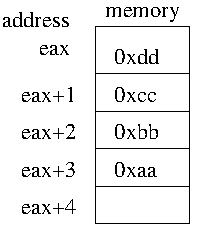
\includegraphics[scale=.7]{fig/memvsarray-1}
\label{endian:membefore}
}
\subfloat[][]{
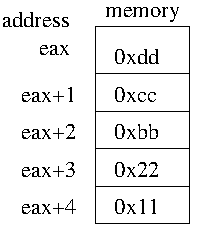
\includegraphics[scale=.7]{fig/memvsarray-2}
\label{endian:memafter}
}
%\end{subfigure}
%\end{minipage}
\caption{(a) shows an example of little-endian stores as found in x86 that
  partially overlap. (b) shows memory after executing line 1, and (c)
  shows memory after executing line 5. Line 7 will load the value 0x22bb.}
\label{fig:endian}
\end{figure}

\section{Normalized Memory} 
\label{vine:normalized}

The endianness of a machine is usually specified by the byte-ordering
of the hardware.  Little endian architectures such as x86 put the
low-order byte first. Big-endian architecture put the high-order byte
first. Some architectures, such as ARM, allow the endianness to be
specified by the instruction, e.g., {\tt mov} would take three
arguments: the source, destination, and endianness for which to
perform the move.


We must take endianness into account when analyzing memory
accesses. Consider the assembly in Figure~\ref{endian:code}. The {\tt
  mov} operation on line 2 writes 4 bytes to memory in little endian
order (since x86 is little endian). After executing line 2, the
address given by {\tt eax} contains byte {\tt 0xdd}, {\tt eax+1}
contains byte {\tt 0xcc}, and so on, as shown in
Figure~\ref{endian:membefore}. Lines 2 and 3 set {\tt ebx =
  eax+2}. Line 4 and 5 write the 16-bit value {\tt 0x1122} to {\tt
  ebx}.  An analysis of these few lines of code needs to consider that
the write on line 4 overwrites the last byte written on line 1, as
shown in Figure~\ref{endian:memafter}. Considering such cases requires
additional logic in each analysis. For example, the value loaded on
line 7 will contain one byte from each of the two stores.

%  In normalized memory,
% all addresses are of the same type $\tau_{\text{addr}} \in
% \tau_{\text{reg}}$, and all values are of type {\tt reg8\_t}.

\begin{figure}
\begin{footnotesize}
\begin{code}  
1. mem4 = let mem1 = store(mem0,eax, 0xdd, 0, reg8\_t) in 
           let mem2 = store(mem1, eax+1, 0xcc, 0, reg8\_t) in 
           let mem3 = store(mem2, eax+2, 0xbb, 0, reg8\_t) in 
               store(mem3, eax+3, 0xcc, 0, reg8\_t);
...
5. mem6 = let mem5 = store(mem4, ebx, 0x22, 0, reg8\_t) in 
             store(mem5, ebx+1, 0x22, 0, reg8\_t) 
...
7. value = let b1 = load(mem6, ebx, 0, reg8\_t) in
            let b2 = load(mem6, ebx+1, 0, reg8\_t) in 
            let b1' = cast(unsigned, b1, 0, reg16\_t) in 
            let b2' = cast(unsigned, b2, 0, reg16\_t) in 
               (b2' $\ll$ 8) $|$ b1';
\end{code}
\end{footnotesize}
\caption{Normalized version of the store and load from Figure~\ref{endian:code}.}
\label{endian:normalized}
\end{figure}


We say a memory is \emph{normalized} for a $b$-byte addressable memory
if all loads and stores are exactly $b$-bytes and $b$-byte
aligned. In x86, memory is byte addressable, so a
normalized memory for x86 has all loads and stores at the byte
level. The normalized form for the write on Line 1 of
Figure~\ref{endian:code} in \bil is shown in
Figure~\ref{endian:normalized}.  Note that the subsequent load on line 7
is with respect to the current memory {\tt mem6}.

Normalized memory makes writing program analyses involving memory
easier.  Analysis is easier because normalized memory syntactically
exposes memory updates that are otherwise implicitly defined by the
endianness.  As a result, analyses do not have to reason explicitly
about overlapping memory, byte order, etc. \bap provides utilities for
normalizing all memory operations so that users can write analysis
more easily.



% Endianness can complicate analysis. 
% specified bit-ordering of the hardware, i.e., a specification of which
% hardware bit corresponds to the low-order bit in a number. 

% Assembly memory operations are
% performed with respect to the endianness (byte ordering) of the
% hardware. 

% A memory operation may either be little endian or big
% endian. A little endian operation to address $a$ stores the low-order
% byte in a register in the lowest memory address, the next lowest-order
% byte in the



% We provide routines to conver little and big endian memories to
% normalized form. The advantage of normalized memory is it eases
% analysis.  For example, consider the x86 instruction sequence shown
% in Figure~\ref{fig:memvsarray}.

% Instruction 1 stores the value 0xaabbccdd into the address given by
% {\tt \%eax}. Since x86 is little-endian, the bytes are stored in
% memory from lowest to highest, as shown in Figure~\ref{fig:}.

% which stores the value in the 4-byte {\tt \%ebx} register
% into the address given by {\tt \%eax}. This instruction on x86 is
% syntatic sugar for storing the low-order byte of {\tt \%ebx} at
% address {\tt \%eax}, the second low-order byte in {\tt \%eax+1}, the
% third in {\tt \%eax+2}, and the high-order byte in {\tt \%eax+3}. In
% \bap, a normalized memory desugars such statements, so {\tt mov
%   *\%eax, \%ebx} becomes:
% \begin{footnotesize}
% \begin{code}
%   // mov *\%eax, \%ebx is desugared in normalized vine memory as
%     mem1 = store(mem0, eax,   ebx \& 0x000000ff);
%     mem2 = store(mem1, eax+1, ebx \& 0x0000ff00);
%     mem3 = store(mem2, eax+2, ebx \& 0x00ff0000);
%     mem4 = store(mem3, eax+3, ebx \& 0xff000000);
% \end{code}
% \end{footnotesize}


% Typically an assembly program works on a single memory.  

% Values in \bap are either register values or memories.  

% Scalar variables in \bap roughly correspond to registers. Although

% In this section we describe the \bap IL.  We first present the \bap
% IL.  In \bap, we have several statements that are derived
% forms. These derived forms are a ``syntatic sugar'' that make writing
% analysis easier, though add no real power to the language.  As
% mentioned, one of the principles of \bap is to treat assembly as a
% first class language. One consequence is \bap does not have
% functions. However, we have observed that several analysis benefit
% from assuming functions exist. We present \bap$_f$, which is an
% extension to \bap which includes functions.



% subsection

%\subsection{\bap and the Running Example}

\begin{figure}
\begin{minipage}[c]{.45\linewidth}
  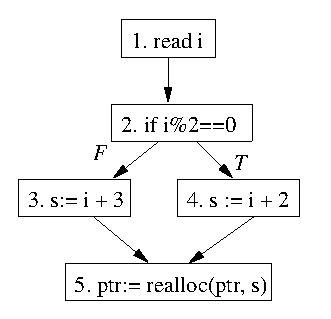
\includegraphics{fig/running-example}
  \label{vine:running-example-fig}
\end{minipage}
\begin{scriptsize}
\begin{minipage}[c]{.45\linewidth}
\begin{lstlisting}
// address instr dst, src
0x8048419 push   ebp  // setup stack
0x804841a mov    ebp,esp
0x804841c sub    esp, 0x18
0x804841f lea    eax, [ebp-0x8]
0x8048422 mov    [esp], eax 
0x8048425 call   0x80483f4 // call read
0x804842a mov    eax, [ebp-0x8]
0x804842d and    eax, 0x1  // if i%2==0
0x8048430 test   eax,eax
0x8048432 jne    0x804843f
0x8048434 mov    eax,[ebp-0x8]
0x8048437 add    eax, 0x2  // s := i+2
0x804843a mov    [ebp-0x4], eax
0x804843d jmp    0x8048448
0x804843f mov    eax,[ebp-0x8]
0x8048442 add    eax,0x3  // s := i+3
0x8048445 mov    [ebp-0x4], eax
0x8048448 mov    eax, [ebp-0x4]
0x804844b mov    [esp+0x4], eax
0x804844f mov    eax, [ebp+0x8]
0x8048452 mov    [esp],eax
0x8048455 call   0x8048338 // call realloc
0x804845a mov    [ebp+0x8],eax
0x804845d leave  
0x804845e ret    
\end{lstlisting}
\end{minipage}
\end{scriptsize}
\caption{Our running example from \ref{intro:running} on the  left, and the
  corresponding x86 assembly in Intel syntax on the right.}
\label{fig:running-asm}
\end{figure}

% \begin{figure}
% \begin{scriptsize}
% \begin{minipage}[c]{.45\linewidth}
% \begin{lstlisting}
% 0x8048419 push   ebp
% 0x804841a mov    ebp,esp
% 0x804841c sub    esp, 0x18
% 0x804841f lea    eax, [ebp-0x8]
% 0x8048422 mov    [esp], eax
% 0x8048425 call   0x80483f4
% 0x804842a mov    eax, [ebp-0x8]
% 0x804842d and    eax, 0x1
% 0x8048430 test   eax,eax
% 0x8048432 jne    0x804843f
% 0x8048434 mov    eax,[ebp-0x8]
% 0x8048437 add    eax, 0x2
% \end{lstlisting}
% \end{minipage}
% \begin{minipage}[c]{.45\linewidth}
% \begin{lstlisting}
% 0x804843a mov    [ebp-0x4], eax
% 0x804843d jmp    0x8048448
% 0x804843f mov    eax,[ebp-0x8]
% 0x8048442 add    eax,0x3
% 0x8048445 mov    [ebp-0x4], eax
% 0x8048448 mov    eax, [ebp-0x4]
% 0x804844b mov    [esp+0x4], eax
% 0x804844f mov    eax, [ebp+0x8]
% 0x8048452 mov    [esp],eax
% 0x8048455 call   0x8048338
% 0x804845a mov    [ebp+0x8],eax
% 0x804845d leave  
% 0x804845e ret    
% \end{lstlisting}
% \end{minipage}
% \end{scriptsize}
% \caption{The running example from Figure~\ref{vine:running-example-fig} in
%   Intel-syntax x86 assembly.}
% \label{fig:running-asm}
% \end{figure}


%\begin{figure}
\begin{scriptsize}
\begin{minipage}[c]{.50\linewidth}
\begin{lstlisting}
label 0x8048419; //push   ebp
  ESP = ESP - 4;
  mem = store(mem, ESP, EBP, reg32_t);
label 0x804841a; //mov    ebp,esp
  EBP = ESP;
label 0x804841c; //sub esp, 0x18
  ESP = ESP-24; 
  /* 'sub' eflags omitted */
label 0x804841f; //lea    eax, [ebp-0x8]
  EAX = (EBP+0xFFFFFFF8);
label 0x8048422; //mov    [esp], eax
  mem = store(mem, ESP, EAX, reg32_t);
label 0x8048425; //call   0x80483f4
  ESP = ESP-4;
  mem = store(mem, ESP, 0x804842A, reg32_t);
  jmp(0x80483f4); 
label 0x804842a; //mov    eax, [ebp-0x8]
  EAX = load(mem, EBP+0xFFFFFFF8,reg32_t);
label 0x804842d; //and    eax, 0x1
  EAX = EAX & 1; 
  /* 'and' eflags omitted */
label 0x8048430; //test   eax,eax
  temp = EAX & EAX;
  ZF:reg1_t = temp == 0; 
  /* SF and PF code omitted */
label 0x8048432; //jne    0x804843f
  cjmp(ZF,0x8048434,0x804843F);
label 0x8048434; //mov    eax,[ebp-0x8]
  EAX = load(mem, EBP+0xFFFFFFF8, reg32_t);
label 0x8048437; //add    eax, 0x2 
  EAX = EAX + 2; 
  /* 'add' eflags omitted */
\end{lstlisting}
\end{minipage}
\begin{minipage}[c]{.45\linewidth}
\begin{lstlisting}
label 0x804843a; //mov    [ebp-0x4], eax
  mem = store(mem, EBP+0xFFFFFFFC, EAX, reg32_t);
label 0x804843d; //jmp    0x8048448
  jmp(0x8048448);
label 0x804843f; //mov    eax,[ebp-0x8]
  EAX = load(mem, EBP+0xFFFFFFF8, reg32_t);
label 0x8048442; //add    eax,0x3
  EAX = EAX+3; 
  /* 'add' eflags omitted */
label 0x8048445; //mov    [ebp-0x4], eax
  mem = store(mem, EBP+0xFFFFFFFC, EAX, reg32_t);
label 0x8048448; //mov    eax, [ebp-0x4]
  EAX = load(mem, EBP+0xFFFFFFFC, reg32_t);
label 0x804844b; //mov    [esp+0x4], eax
  mem = store(mem, ESP+4, EAX, reg32_t);
label 0x804844f; //mov    eax, [ebp+0x8]
  EAX = load(mem, EBP+8, reg32_t);
label 0x8048452; //mov    [esp],eax
  mem = store(mem, ESP, EAX, reg32_t);
label 0x8048455; //call   0x8048338
  ESP = ESP-4;
  mem = store(mem, ESP, 0x804845A, reg32_t);
  jmp(0x8048338); 
label 0x804845a; //mov    [ebp+0x8],eax
  mem = store(mem, ESP+8, EAX, reg32_t);
label 0x804845d; //leave
  ESP = EBP+4;
  EBP = load(mem, EBP, reg32_t);
label 0x804845e; //ret
  target = load(mem, ESP, reg32_t);
  ESP = ESP+4;
  jmp(target);
\end{lstlisting}
\end{minipage}
\end{scriptsize}
\caption{The assembly from Figure~\ref{fig:running-asm} in the \bap IL.}
\label{fig:running-il}
\end{figure}

Figure~\ref{fig:running-asm} shows the assembly for the running
example from \chref~1 (which is reproduced as part of the figure). The
assembly (given in Intel syntax) shown is for the running example
compiled as a single function which is passed in {\tt ptr}, with {\tt
read} and {\tt realloc} as external calls.  Each assembly line
contains the instruction address followed by the instruction with
operands.

The first 4 instructions in Figure~\ref{fig:running-asm} implement the
function prologue, which sets up the stack frame.  The variable {\tt i}
is assigned by the compiler to register {\tt eax}. Instruction
0x804822-0x804825 push the argument {\tt eax} onto the stack, and then
call the function corresponding to {\tt read} at address 0x80483f4.
Instruction 0x804842d-0x8048430 correspond to the test {\tt if i \%2
== 0}.  The compiler implemented the reduction modulo 2 as bit-wise ``and''.
Instructions 0x8048437-0x804843d implement the true branch where {\tt
s := i+2}.  The compiler assigned the variable {\tt s} the register
{\tt eax} in assembly, which is put on the local stack frame slot {\tt
ebp-0x4}.  Instructions 0x8048442-0x8048445 implement the false branch
where {\tt s := i+3}, again storing the result in {\tt ebp-0x4}.  Line
0x804844b-0x48455 correspond to the call to {\tt realloc}, followed by
the function epilogue.

\begin{figure}
\begin{scriptsize}
\begin{minipage}[c]{.50\linewidth}
\begin{lstlisting}
label 0x8048419; //push   ebp
  ESP = ESP - 4;
  mem = store(mem, ESP, EBP, reg32_t);
label 0x804841a; //mov    ebp,esp
  EBP = ESP;
label 0x804841c; //sub esp, 0x18
  ESP = ESP-24; 
  /* 'sub' eflags omitted */
label 0x804841f; //lea    eax, [ebp-0x8]
  EAX = (EBP+0xFFFFFFF8);
label 0x8048422; //mov    [esp], eax
  mem = store(mem, ESP, EAX, reg32_t);
label 0x8048425; //call   0x80483f4
  ESP = ESP-4;
  mem = store(mem, ESP, 0x804842A, reg32_t);
  jmp(0x80483f4); 
label 0x804842a; //mov    eax, [ebp-0x8]
  EAX = load(mem, EBP+0xFFFFFFF8,reg32_t);
label 0x804842d; //and    eax, 0x1
  EAX = EAX & 1; 
  /* 'and' eflags omitted */
label 0x8048430; //test   eax,eax
  temp = EAX & EAX;
  ZF:reg1_t = temp == 0; 
  /* SF and PF code omitted */
label 0x8048432; //jne    0x804843f
  cjmp(ZF,0x8048434,0x804843F);
label 0x8048434; //mov    eax,[ebp-0x8]
  EAX = load(mem, EBP+0xFFFFFFF8, reg32_t);
label 0x8048437; //add    eax, 0x2 
  EAX = EAX + 2; 
  /* 'add' eflags omitted */
\end{lstlisting}
\end{minipage}
\begin{minipage}[c]{.45\linewidth}
\begin{lstlisting}
label 0x804843a; //mov    [ebp-0x4], eax
  mem = store(mem, EBP+0xFFFFFFFC, EAX, reg32_t);
label 0x804843d; //jmp    0x8048448
  jmp(0x8048448);
label 0x804843f; //mov    eax,[ebp-0x8]
  EAX = load(mem, EBP+0xFFFFFFF8, reg32_t);
label 0x8048442; //add    eax,0x3
  EAX = EAX+3; 
  /* 'add' eflags omitted */
label 0x8048445; //mov    [ebp-0x4], eax
  mem = store(mem, EBP+0xFFFFFFFC, EAX, reg32_t);
label 0x8048448; //mov    eax, [ebp-0x4]
  EAX = load(mem, EBP+0xFFFFFFFC, reg32_t);
label 0x804844b; //mov    [esp+0x4], eax
  mem = store(mem, ESP+4, EAX, reg32_t);
label 0x804844f; //mov    eax, [ebp+0x8]
  EAX = load(mem, EBP+8, reg32_t);
label 0x8048452; //mov    [esp],eax
  mem = store(mem, ESP, EAX, reg32_t);
label 0x8048455; //call   0x8048338
  ESP = ESP-4;
  mem = store(mem, ESP, 0x804845A, reg32_t);
  jmp(0x8048338); 
label 0x804845a; //mov    [ebp+0x8],eax
  mem = store(mem, ESP+8, EAX, reg32_t);
label 0x804845d; //leave
  ESP = EBP+4;
  EBP = load(mem, EBP, reg32_t);
label 0x804845e; //ret
  target = load(mem, ESP, reg32_t);
  ESP = ESP+4;
  jmp(target);
\end{lstlisting}
\end{minipage}
\end{scriptsize}
\caption{The assembly from Figure~\ref{fig:running-asm} in the \bap IL.}
\label{fig:running-il}
\end{figure}

Figure~\ref{fig:running-il} shows the \bap IL for the assembly in
Figure~\ref{fig:running-asm}. For simplicity, we note where {\tt
eflags} code is calculated, but do not include the logic in the
Figure. Each assembly instruction is lifted in a syntax-directed
manner.

The IL reduces complex x86 instructions to a simplified language. For
example, the x86 {\tt push ebp} instruction at 0x8048419 in the IL is
de-sugared as decrementing the register {\tt esp} by one word, then
storing {\tt ebp} at the resulting address in memory.  Another example
is in assembly, there is no syntactic relationship between the {\tt
test} instruction at 0x8048430 and the conditional jump {\tt jne} at
0x804843f. The IL, however, explicitly shows {\tt test} sets the {\tt
 ZF} flag, which the raised conditional jump checks.



% subsection
%\input{derived}
% subsection
%\subsection{\bap Typing}
\label{vinesec:typecheck}

%\renewcommand{\baselinestretch}{1.0}\normalsize

\begin{table}

{\bf Context}\\
\begin{tabular}{llp{4.5in}}
$\Gamma$ & \emphkind{var} $\rightarrow$ $\tau$& 
Typing context of $(x:\tau)$ pairs where $x$ is of type $\tau$.
\end{tabular}\\[10pt]
{\bf Program and Instructions}
\begin{footnotesize}
\[
\begin{array}{c}
\infer[]
 { 
   \cdot \vdash (x_i:\tau_i)^* i^*  : ()
 }
 {
   \forall i \in i^* | (x_i:\tau_i)^* \vdash i : ()
 }
\end{array}
\]
\[
\begin{array}{ccc}
\infer[\textsc{assign}]
   {
     \Gamma \vdash x := e : ()
   }
   {
     \Gamma \vdash e : \tau
     &
     \Gamma \vdash x : \tau
   } &
\infer[\textsc{jmp}]
   {
     \Gamma \vdash \texttt{jmp($e$)} : ()
   }
   {
     \Gamma \vdash e : \texttt{reg64\_t}
   } & 
\infer[\textsc{halt}]
  {
     \Gamma \vdash \texttt{halt($e$)} : ()
  }
  { 
     \Gamma \vdash e : \tau
     & \tau \in \tau_{\text{reg}}
  }
\end{array}
\]
\[
\begin{array}{c}
\infer[\textsc{cjmp}]
   {
     \Gamma \vdash \texttt{cjmp($e_1$, $e_2$, $e_3$)} : ()
   }
   {
      \Gamma \vdash e_1 : \texttt{reg1\_t}
      & 
      \Gamma \vdash e_2 : \texttt{reg64\_t}
      &
      \Gamma \vdash e_3 : \texttt{reg64\_t}
   }
\end{array}
\]
\[
\begin{array}{ccc}
\infer[\textsc{assert}]
  {
    \Gamma \vdash \texttt{assert($e$)} : ()
  }
  {
    \Gamma \vdash e : \texttt{reg1\_t}
  } &
 \infer[\textsc{label}]
  {
    \Gamma \vdash \texttt{label $n$} : ()
  }
  {
  } &
\infer[\textsc{special}]
  {
   \Gamma \vdash \texttt{special {\sf id$_s$}} : ()
  }
  {
  }
\end{array}
\]
\end{footnotesize}
{\bf Auxiliary Definitions}
\begin{footnotesize}
\[
\begin{array}{c}
 \infer[\textsc{reg-subtype}]
   {
     \texttt{reg1\_t $<:$ reg8\_t $<:$ reg16\_t $<:$ reg32\_t $<:$ reg64\_t}
   }
   {
   }
\end{array}
\]
\[
\begin{array}{cc}
\infer[]
  {
    \text{mem\_compat($\tau_1$, $\tau_2$)}
  }
  {
   \tau_1 = \texttt{big $|$ little} 
    & \tau_2 \in \tau_{\text{reg}} 
  } &
\infer[]
  {
    \text{mem\_compat({\tt norm}, {\tt reg8\_t})}
  }
  {
  }\\[10pt]
\infer[]
  {
    \text{cast\_compat(k, $\tau_1$, $\tau_2$)}
  }
  {
    k = \texttt{unsigned $|$ signed}
    & 
    \tau_1 <: \tau_2
  }&
\infer[]
  {
    \text{cast\_compat(k, $\tau_1$, $\tau_2$)}
  }
  {
    k = \texttt{hi $|$ low}
    & 
    \tau_2 <: \tau_1
  }
\end{array}
\]
\end{footnotesize}
{\bf Expressions}
\begin{footnotesize}
\[
\begin{array}{cc}
\infer[\textsc{load}]
  { % conclusion
    \Gamma \vdash \texttt{load($e_1$, $e_2$, $\tau$)} : \tau
  }
  { % premise
    \Gamma \vdash e_1 : \texttt{mem\_t($\tau_1$, $\tau_2$)}
    & 
    \text{mem\_compat($\tau_1$, $\tau$)}
    &
    \Gamma \vdash e_2 : \tau_2
  } &
\infer[\textsc{var}]
  { % conclusion
      \Gamma \vdash x : \tau
  }
  { % premise
        x:\tau \in \Gamma
  }
\end{array}
\]
\[
\begin{array}{c}
\infer[\textsc{store}]
  { % conclusion
    \Gamma \vdash \texttt{store($e_1$, $e_2$,$e_3$)}:\texttt{mem\_t($\tau_1$, $\tau_2$)}
  }
  { %premise
    \Gamma \vdash e_1: \texttt{mem\_t($\tau_1$, $\tau_2$)}
    &
    \Gamma \vdash e_2 : \tau_2 
    & 
    \Gamma \vdash e_3 : \tau_4
    & 
    \text{mem\_compat($\tau_1$, $\tau_4$)}
  }\\
\end{array}
\]
\[
\begin{array}{cc}
\infer[\textsc{binop$_1$}]
  { % conclusion
    \Gamma \vdash e_1 \Diamond_b e_2 : \tau
  }
  { % premise
    \Gamma \vdash e_1 : \tau 
    & \Gamma \vdash e_2 : \tau
    & \tau \in \tau_{\text{reg}}
    & \Diamond_b \notin \ll, \gg, \gg_a
  } &
\infer[\textsc{unop}]
  { % conclusion
    \Gamma \vdash \Diamond_u e : \tau
  }
  { % premise
    \Gamma \vdash e : \tau 
    & \tau \in \tau_{\text{reg}}
  } 
\end{array}
\]
\[
\begin{array}{c}
\infer[\textsc{binop$_2$}]
  { % conclusion
    \Gamma \vdash e_1 \Diamond_b e_2 : \tau
  }
  { % premise
    \Gamma \vdash e_1 : \tau 
    & \Gamma \vdash e_2 : \tau_2
    & \tau, \tau_2 \in \tau_{\text{reg}}
    & \Diamond_b \in \ll, \gg, \gg_a
  } 
\end{array}
\]
\[
\begin{array}{cc}
\infer[\textsc{cast}]
  { % conclusion 
   \Gamma \vdash \texttt{cast(\emphkind{cast\_kind}, $\tau$, $e$)} : \tau
  }
  { % premise
    \Gamma \vdash e : \tau_1
    & \tau, \tau_1 \in \tau_{\text{reg}}
    & \text{cast\_compat(\emphkind{cast\_kind}, $\tau_1$, $\tau$)}
  } &
\infer[\textsc{let}]
  { % conclusion
    \Gamma \vdash \texttt{let $x$ := $e_1$ in $e_2$} : \tau
  }
  { % premise
    \Gamma \vdash e_1 : \tau_1
    & \Gamma,(x:\tau_1) \vdash e_2 : \tau
  } 

\end{array}
\]
\end{footnotesize}
\caption{Type-checking rules for \bap.}
\label{vine:typecheck}
\end{table}
%\renewcommand{\baselinestretch}{1.66}\normalsize


The \bap IL syntax described in Table~\ref{vine:syntax} is designed
to be simple. A literal interpretation, however, allows several
nonsensical operations such as left-shifting two memory variables.  We
type-check \bap programs using the  rules shown in
Table~\ref{vine:typecheck} to weed out obviously nonsensical
operations.  We emphasize that type-checking to show program safety is outside
the scope of \bap.

The type-checking rules are straight-forward.  \bap requires that
binary and unary operations be on scalars of the same register type
(except shifts where the shift amount need only be an integer). We
type-check {\tt hi} and {\tt low} casts such that the resulting type
is a smaller register type (in terms of the sub-typing relationship
{\sc reg-subtype}), as expected.  {\tt unsigned} and {\tt signed}
casts must be to a wider register type. One issue with un-normalized
memory is that it may have multi-byte accesses, e.g., a store on x86
could be of 32, 16, or 8 bits. Normalized memory, on the other hand,
only allows stores and loads of bytes.  We define an auxiliary
predicate ``mem\_compat'' to ensure that normalized memory is accessed
appropriately.  Also note that as a convenience we assume 64-bit
addressing in the rules, but allow smaller addressable memories via
the {\tt reg-subtype} sub-typing rule.

A program type-checks if all instructions type-check under the
declared variable types.  We require all variables be declared because
explicitly typed languages are easier to check. 


% subsection
\section{Operational Semantics}
\label{vine:operational}


%\renewcommand{\baselinestretch}{1.0}\normalsize

\begin{table}
{\bf Contexts}\\
\begin{tabular}{lllp{4in}}
  {\it Statement} & $\Pi$ & $n$ $\mapsto$ \emphkind{instr} &
  Maps an statement address to an statement.\\
  {\it Variable} & $\Delta$ &  $id \mapsto \emphkind{var}$  &Maps
  a variable ID to its value.\\
  {\it Labels} & $\Lambda$ & $\emphkind{label\_kind} \mapsto n$ & Maps
  a label to the address of the corresponding {\tt label} statement number.
\end{tabular}\\
\newline
{\bf Notation}\\
\begin{tabular}{lp{4.2in}}
  $\Delta \vdash e \Downarrow v$ & Expression $e$ evaluates to value
  $v$ given variable context $\Delta$ as given by the expression
  evaluation rules.\\
  $\Delta' = \Delta[x \leftarrow v]$ & $\Delta'$ is the same as
  $\Delta$ except extended to map $x$  to $v$.\\
  $\Pi \vdash p:s$ & $\Pi$ maps statement address $p$ to statement
  $s$. If $p \notin \Pi$, the machine gets stuck.\\
  $\Lambda \vdash v:p$ & $\Lambda$ maps statement label $v$ to statement
  address $p$. If $v \notin \Lambda$, then machine gets stuck. In
  addition, a well-formed machine should have $\Pi \vdash p : s$
  where $s = \texttt{label $v$}$, otherwise the machine is stuck.\\
%   $(\Pi, \Delta, p, \iota)$ & An abstract machine configuration.
%   $\Pi$ and $\Delta$ are contexts define above, $p$ is the program
%   counter, and $\iota$ is the current statement.\\  
  $(\Delta, p, s) \leadsto (\Delta', p', s')$ &  An
  execution step. $p$ and $p'$ are
  the pre and post step program counters, $s$ and $s'$ are the pre and
  post step  statements, and $\Delta$ and $\Delta'$ are the pre and post
  step variable contexts. Note $\Lambda$ and $\Pi$ are currently static, thus
  for brevity not included in the execution context.\\
\end{tabular}
\caption{Operational Semantics Notation.}
\end{table}

\begin{table}
{\bf Statements}
\begin{small}
\[
\begin{array}{cc}
  \infer[\textsc{Assign}]
    { % conclusion
      \Delta, p, \text{x := $e$} 
      \leadsto 
      \Delta', p+1, s
    }
    { % premise
      \Delta \vdash e \Downarrow v 
      & \Delta' = \Delta[x \leftarrow v]
      & \Pi \vdash p+1:s
    } &
  \infer[\textsc{Jmp}]
  { % conclusion
    \Delta, p, \texttt{jmp($\ell$)} 
    \leadsto 
    \Delta, p', \texttt{label $v$}
  }
  { % premise
    \Delta \vdash \ell \Downarrow v
    & \Lambda \vdash v : p'
    & \Pi \vdash p' : \texttt{label $v$}
  }\\[10pt]
  \infer[\textsc{label}]
  { % conclusion
    \Delta, p, \texttt{label $\ell$} 
    \leadsto
    \Delta, p+1, s
  }
  { % premise
      \Pi \vdash p+1:s
  } &
  \infer[\textsc{halt}]
  { % conclusion
    \Delta, p, \texttt{halt $e$} 
    \leadsto
    \text{terminate with  $v$}
%    \Pi, \Delta, p+1, \texttt{halt $v$}
  }
  {
     \Delta \vdash e \Downarrow v
  }\\[10pt]
  \infer[\textsc{assert-t}]
  { % conclusion
    \Delta, p, \texttt{assert}(e)
    \leadsto
    \Delta, p+1, s
  } 
  { % premise
    \Delta \vdash e \Downarrow 1 &
    \Pi \vdash p+1:s
  } &
  \infer[\textsc{assert-f}]
  { % conclusion
    \Delta, p, \texttt{assert}(e)
    \leadsto
    \text{terminate with  $\perp$}
  }
  { % premise
    \Delta \vdash e \Downarrow 0
  }
\\
\end{array}
\]
\[
\begin{array}{c}
  \infer[\textsc{CJmp-t}]
  { %conclusion
    \Delta, p, \texttt{cjmp($e$, $\ell_T$, $\ell_F$)} 
    \leadsto
    \Delta, p',  \texttt{label $v$}
  }
  { %premise
    \Delta \vdash e \Downarrow 1
    & \Delta \vdash \ell_T \Downarrow v
    & \Lambda \vdash v: p'
    & \Pi \vdash p' :  \texttt{label $v$}
  }\\[10pt]
  \infer[\textsc{CJmp-f}]
  { %conclusion
    \Delta, p, \texttt{cjmp($e$, $\ell_T$, $\ell_F$)} 
    \leadsto
    \Delta, p', \texttt{label $v$}
  }
  { %premise
    \Delta \vdash e \Downarrow 0
    & \Delta \vdash \ell_F \Downarrow v
    & \Lambda \vdash v: p'
    & \Pi \vdash p' : \texttt{label $v$}
  } \\[10pt]
  \text{No rule for {\tt special}, when
    $v \notin \Lambda$, and when  $p \notin \Pi$.}  
\end{array}
\]
\end{small}
\caption{Operational Semantics of Statements.}
\label{bap:taboperstmts}
\end{table}

\begin{table}
{\bf Expressions}\\
\begin{small}
\[
\begin{array}{cc}
  \infer[\textsc{binop}]
  { % conclusion
    \Delta \vdash e_1 \Diamond_b e_2 \Downarrow v
  }
  { % premise
    \Delta \vdash e_1 \Downarrow v_1 
    & \Delta \vdash e_2 \Downarrow v_2
    & v = v_1 \Diamond_b v_2
  } &
  \infer[\textsc{unop}]
  { % conclusion
    \Delta \vdash \Diamond_u e_1 \Downarrow v
  } 
  { % premise
    \Delta \vdash e_1 \Downarrow v_1 
    & v = \Diamond_u v_1
  }\\[10pt]
\end{array}
\]
\[
\begin{array}{ccc}
  \infer[\textsc{Value}]
  { % conclusion
    \Delta \vdash v \Downarrow v
  } 
  { % premise (empty)
  } &
  \infer[\textsc{Var}]
  { % conclusion
    \Delta \vdash x \Downarrow v
  }
  { % premise
    \Delta \vdash x:v
  } &
  \infer[\textsc{let}]
  { % conclusion
    \Delta \vdash \texttt{let $x$ = $e_1$ in $e_2$} \Downarrow v
  }
  { % premise
    \Delta \vdash e_1 \Downarrow v_1 
    & \Delta' = \Delta[x \leftarrow v_1]
    & \Delta' \vdash e_2 \Downarrow v
  }\\
\end{array}
\]
\[
\begin{array}{c}
  \infer[\textsc{Load$_{\text{little}}$}]
  { % conclusion
    \Delta \vdash \texttt{load($e_1$, $e_2$, $e_3$, $\tau_{\text{reg}}$)} \Downarrow v
  }
  { % premise
    \Delta \vdash e_1 \Downarrow v_1 
    & \Delta \vdash e_2 \Downarrow v_2
    & \Delta \vdash e_3 \Downarrow 0
    & n = \text{\# bytes of $\tau_{\text{reg}}$}
    & v = v_1[v_2..v_2+n] \text{ in little endian byte order}
  } \\[10pt]
  \infer[\textsc{Load$_{\text{big}}$}]
  { % conclusion
    \Delta \vdash \texttt{load($e_1$, $e_2$, $e_3$, $\tau_{\text{reg}}$)} \Downarrow v
  }
  { % premise
    \Delta \vdash e_1 \Downarrow v_1 
    & \Delta \vdash e_2 \Downarrow v_2
    & \Delta \vdash e_3 \Downarrow 1
    & n = \text{\# bytes of $\tau_{\text{reg}}$}
    & v = v_1[v_2..v_2+n] \text{ in big endian byte order}
  } \\[10pt]
  \infer[\textsc{Load$_\text{array}$}]
  { % conclusion
    \Delta \vdash \texttt{load($e_1$, $e_2$, $e_3$, \texttt{array\_t})} \Downarrow v
  }
  { % premise
    \Delta \vdash e_1 \Downarrow v_1 
    & \Delta \vdash e_2 \Downarrow v_2
    & \Delta \vdash e_3 \Downarrow 0
    & v = v_1[v_2]
  } \\[10pt]
  \infer[\textsc{Store$_{\text{little}}$}]
  { % conclusion
    \Delta \vdash \texttt{store($e_1$, $e_2$, $e_3$, $e_4$, $\tau_{\text{reg}}$)}  \Downarrow v
  }
  { % premise
    \Delta \vdash e_1 \Downarrow v_1 
    & \Delta \vdash e_2 \Downarrow v_2
    & \Delta \vdash e_3 \Downarrow v_3
    & \Delta \vdash e_4 \Downarrow 0
    & n = \text{\# bytes $\tau_{\text{reg}}$}
    & v = v_1[v_2..v_2+n \leftarrow v_3] \text{ (little endian)}
  }\\[10pt]
  \infer[\textsc{Store$_{\text{big}}$}]
  { % conclusion
    \Delta \vdash \texttt{store($e_1$, $e_2$, $e_3$, $e_4$, $\tau_{\text{reg}}$)}  \Downarrow v
  }
  { % premise
    \Delta \vdash e_1 \Downarrow v_1 
    & \Delta \vdash e_2 \Downarrow v_2
    & \Delta \vdash e_3 \Downarrow v_3
    & \Delta \vdash e_4 \Downarrow 1
    & n = \text{\# bytes $\tau_{\text{reg}}$}
    & v = v_1[v_2..v_2+n \leftarrow v_3] \text{ (big endian)}
  }\\[10pt]
  \infer[\textsc{Store$_{\text{array}}$}]
  { % conclusion
    \Delta \vdash \texttt{store($e_1$, $e_2$, $e_3$, $e_4$, \texttt{array\_t})}  \Downarrow v
  }
  { % premise
    \Delta \vdash e_1 \Downarrow v_1 
    & (e_1 : \texttt{array\_t})
    & \Delta \vdash e_2 \Downarrow v_2
    & \Delta \vdash e_3 \Downarrow v_3
    & (e_4 \text{ ignored})
    & v = v_1[v_2 \leftarrow v_3]
  }
\end{array}\\
\]
\[
\begin{array}{cc}
  \infer[\textsc{cast$_u$}]{ %conclusion
    \Delta \vdash \texttt{cast(unsigned, $\tau_{\text{reg}}$, $e$)}
    \Downarrow v
  }
  { %premise
   \Delta \vdash e \Downarrow v & \text{zero extend $v$ to
    $\tau_{\text{reg}}$ bits}
  } &
  \infer[\textsc{cast$_s$}]{ %conclusion
    \Delta \vdash \texttt{cast(signed, $\tau_{\text{reg}}$, $e$)}
    \Downarrow v
  }
  { %premise
   \Delta \vdash e \Downarrow v & \text{sign extend $v$ to
    $\tau_{\text{reg}}$ bits}
  }\\[10pt]
    \infer[\textsc{cast$_h$}]{ %conclusion
    \Delta \vdash \texttt{cast(high, $\tau_{\text{reg}}$, $e$)}
    \Downarrow v
  }
  { %premise
   \Delta \vdash e \Downarrow v & \text{extract 
    $\tau_{\text{reg}}$  high bits of $v$}
  } &
    \infer[\textsc{cast$_l$}]{ %conclusion
    \Delta \vdash \texttt{cast(low, $\tau_{\text{reg}}$, $e$)}
    \Downarrow v
  }
  { %premise
   \Delta \vdash e \Downarrow v & \text{extract 
    $\tau_{\text{reg}}$  low bits of $v$}
  }\\[10pt]
  \infer[\textsc{name}]
  { % conclusion
    \cdot \vdash \texttt{name}\text{(string)} : \text{string}
  }
  { % premise
  } &
  \infer[\textsc{unknown}]
  { % conclusion
    \cdot \vdash \texttt{unknown}(s) \Downarrow \perp
  }
  { % premise
  }
\end{array}
\]
\end{small}
\caption{Operational Semantics of Expressions.}
\label{bap:taboperationalexp}
\end{table}

%\renewcommand{\baselinestretch}{1.66}\normalsize

%%% Local Variables: 
%%% mode: latex
%%% TeX-master: "../main"
%%% End: 


The operational semantics for \bil are shown in
Tables~\ref{bap:taboperstmts} and \ref{bap:taboperexps}.  The abstract
machine configuration is given by the tuple $(\Pi, \Delta, p, s)$
where $\Pi$ is the list of statements, $\Delta$ is the variable
context, $p$ is the statement pointer, and $s$ is the current
statement.  We write $\Delta' = \Delta[x \leftarrow v]$ to indicate
that $\Delta'$ is the same as $\Delta$ except that variable $x$ is
updated with value $v$.  For simplicity, we use $\Delta$ both as a
scalar and a memory context. When ambiguous, such as in the {\sc
  store} rule, we indicate the type of the variable in $\Delta$ in
parentheses. We write $\Pi[p]$ to indicate the statement given by
address $p$.

The operational semantics can be read as follows.  Each step of the
execution is associated with a machine configuration $M = (\Pi,
\Delta, p, s)$.  A transition is given by $M \leadsto M'$ where the
current configuration $M$ matches the left side of $\leadsto$ in the
conclusion (below the horizontal bar), resulting in a state $M'$ to
the right.  The transformation from $M$ to $M'$ is given by the rule
premise (above the horizontal bar). 

{\it Note:} \bap and \bil do not analyze dynamically generated
code. Thus, in a machine state transition $(\Pi, \Delta, p, s)
\rightarrow (\Pi', \Delta, p, s)$, $\Pi = \Pi'$ always. Since $\Pi$
(the list of statements) never changes, we omit $\Pi$ from the rules
for brevity. One could add support for dynamically generated code by
adding rules for updating $\Pi$. 


{\sc assign} and {\sc label} are sequential statements that carry
out the respective operation, then look up and transition to the next
sequential statement $p+1$. The semantics of {\sc label} is a no-op:
we use labels for jump targets.  {\sc assign} updates the variable
context $\Delta$ resulting in a new context $\Delta'$.  As mentioned,
there is no rule for {\tt special}; any program with a {\tt special}
remaining may get stuck.

Control flow is handled by {\tt jmp}%%  (since {\tt cjmp} is a derived
%% form per Chapter~\ref{vine:derived})
%% cjmp is not derived in bap?
. A {\tt jmp} statement
evaluates the jump target $e$ to a value $v$, then looks up the
statement associated with $v$.  The {\sc no-inst} rule terminates
the program in the error state when $v$ is not associated with an
statement. For example, consider the case when a program reads in
user input at location $v$, then issues a jump to $v$.  The user input
will be decoded as statements at run-time.  However, since the
statement comes from user input, we cannot include it in the analysis. In
\bap, we indicate such possibilities by terminating in error.




%\subsubsection{\bap With Functions Operational Semantics}
%
\begin{table}
{\bf Contexts}\\
\begin{tabular}{lllp{2.7in}}

  {\it Functions}&$\Sigma$ & \emphkind{proc} $\mapsto$
  (\emphkind{var} list, \emphkind{var} list, $\Pi_{\text{proc}}$) &
  $\Sigma$ is used for setting up function calls. There are three
  things it keeps track of for each procedure given by \emphkind{proc
    id}. The first item in the tuple is the list of argument
  variables   $[arg_1:\tau_1, \ldots ,arg_i:\tau_i]$. The second is the list of
  variables scoped by the procedure $[x_1:\tau_0, \ldots,
  x_n:\tau_n]$. The third is an instruction map $\Pi_{\text{proc}}$ for the
  procedure. $\Pi_{\text{proc}}$ is only defined on instructions which
  are part of the procedure. Note that we define it this way to
  prevent jumps outside of the procedure.\\
  {\it Instructions} & $\Pi$ & $n$ $\mapsto$ \emphkind{instr}&
  Maps an instruction address to the instruction.\\
  {\it Variables} & $\Delta$ &  
  $id \mapsto (\emphkind{var},bool)$  & As before, $\Delta$ is the
  variable context. We augment the mapping such that we also
  keep track of whether a variable is global or local to the
  function.\\
  {\it Stack} & $\Gamma$ & $[(x_1,id_1), (x_2,id_2), ...,(x_n,id_n)]$& 
  The procedure call stack.  Each procedure call saves the tuple
  $(x_i, id_i)$ where $x_i$ is the variable to assign any returned
  value, and $id_i$ is the next instruction to execute after a return.\\
\end{tabular}\\
\newline
{\bf Notation}\\
\begin{tabular}{lp{3.5in}}
  $\Delta \vdash e \Downarrow v$ & As before, expression $e$ evaluates to value
  $v$ given variable context $\Delta$ as given by the expression
  evaluation rules.\\
  $(\Pi, \Sigma, \Gamma, \Delta, p, i)$ & An abstraction machine
  configuration.  We augment the abstract machine to include a context
  of function declarations $\Sigma$, as well as a stack of return
  addresses $\Gamma$. \\
  $(\Pi, \Sigma, \Gamma, \Delta, p, i) \leadsto (\Pi, \Sigma, \Gamma', \Delta', p', \iota)$ &
  An abstract machine execution step. $\Delta'$ is a (possibly
  updated) variable context, and $\Gamma'$ is a (possibly updated)
  stack context.\\
\end{tabular}
\end{table}


%%% Local Variables: 
%%% mode: latex
%%% TeX-master: "../main"
%%% End: 



\chapter{\bap Development Guide}

\section{\bap Overview}

\begin{figure}
\centering
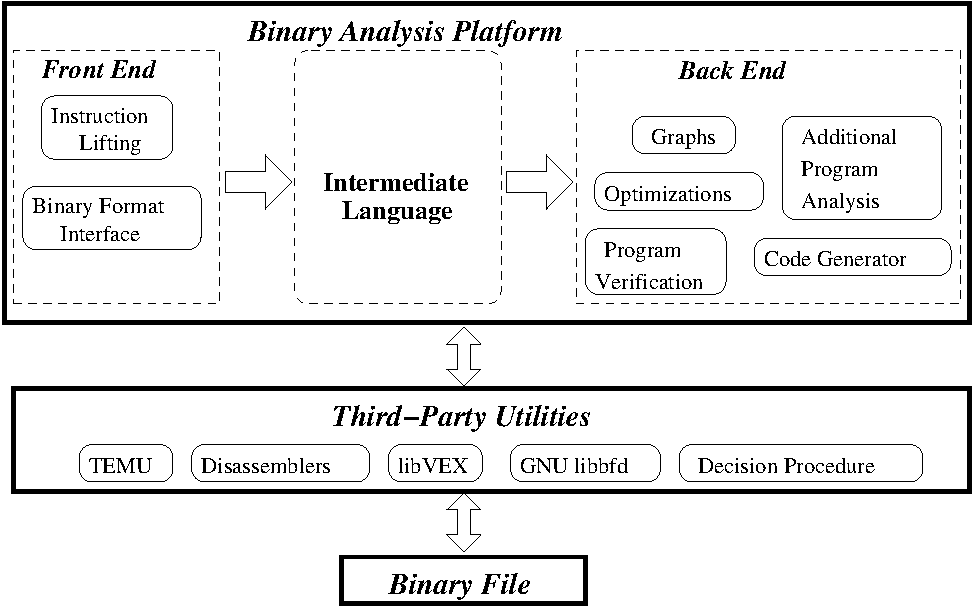
\includegraphics[scale=.8]{fig/components}
\caption{The \bap binary analysis architecture and components. \bap
  is divided into a front-end, which is responsible for lifting
  instructions to the \bap IL, and a platform-independent back-end
  for analyses.}
\label{fig:vine-components}
\end{figure}

\bap  is designed to facilitate faithful
security-relevant binary program analysis by 1) reducing complex
instruction sets to a single, small, and formally specified
intermediate language that supports writing  concise,
easy-to-understand analyses 2) providing a set of core program analyses
abstractions, and 3) being architecture independent when possible in
order to support easy re-targeting.


Figure~\ref{fig:vine-components} shows a high-level picture of \bap.
\bap is divided into an architecture-specific front-end and an
architecture-independent back-end.  At the core of \bap is an
architecture-independent intermediate language (IL), called \emph{\bil,} for
assembly. Assembly instructions in the underlying architecture are
lifted up to the \bil via the \bap front-end.  All analyses are
performed on the platform-independent \bil in the back-end.
%Thus, program analysis can be
%written in an architecture-independent fashion.

We lift to the \bil by using open-source utilities to parse the binary
format and produce assembly.  The assembly is then lifted up to the
\bap IL in a syntax-directed manner. The \bap front-end currently
supports lifting usermode x86~\cite{intel:x86} code, though other
architectures may be added to the \bap framework.
% and ARMv4~\cite{arm:armv4} to the IL.

The \bap back-end supports a variety of core program analyses
and utilities.  The back-end has utilities for creating a variety of
different graphs, such as control flow and program dependence graphs.
The back-end also provides an optimization framework. The optimization
framework is usually used to simplify a specific set of
instructions. We also provide program verification capabilities such
as symbolic execution, calculating the weakest precondition, and
interfacing with decision procedures.  \bap can also write out lifted
\bap instructions as valid C code via the code generator back-end.

%%% Local Variables: 
%%% mode: latex
%%% TeX-master: "../main"
%%% End: 



\chapter{Examples}

In this chapter, we present some hands-on examples that may be useful
to become familiar with BAP's capabilities.

\section{Generating and Working with IL}

One of BAP's central features is the ability to represent the
semantics of binary code in a simple language called BIL (BAP
Intermediate Language).  This example demonstrates how to lift binary
code to the IL and manipulate it in BAP.  Let's start with the
following assembly file:

\verbatiminput{chap-examples/basic.S}

\subsection{Lifting to the IL}

In this form, the program looks very simple.  Let's see what the BAP
representation of the program shows us.  Compile this file (basic.S)
to an object file with \cmdline{gcc -c basic.S -o basic.o}.  We can
lift this object file with BAP's \cmdline{toil} command: \cmdline{toil
  -bin basic.o -o basic.il}. If you inspect \cmdline{basic.il}, you
should see something like:

\verbatiminput{chap-examples/basic.il}

You can see from this example that BAP IL is much more verbose than
assembly; this is on purpose.  It might make BAP IL a little more
tedious to read, but it makes writing analyses much simpler.  Let's go
through some of the IL line by line to explain what is happening.

\begin{verbatim}
addr 0x0 @asm "add    %eax,%ebx"
label pc_0x0
\end{verbatim}
These two statements mark the beginning of a new assembly instruction.
Note the label for pc\_0x0; any jump to address zero will go to to
this label.

\begin{verbatim}
t:u32 = R_EBX:u32
\end{verbatim}
Here we are saving the original value of \%ebx before it is modified.
This original value will be used when computing flags.

\begin{verbatim}
R_EBX:u32 = R_EBX:u32 + R_EAX:u32
\end{verbatim}
This is the primary computation of the add instruction: adding \%eax
to \%ebx.

\begin{verbatim}
R_CF:bool = R_EBX:u32 < t:u32
\end{verbatim}
Here we explicitly compute the value of the carry flag.  After
executing the add instruction, the carry flag is set if the resulting
value of \%ebx is less than the original value of \%ebx (which is
saved in t).

\begin{verbatim}
R_OF:bool =
  if (R_ECX:u32 & 0x1f:u32) == 0:u32 then R_OF:bool else
  if (R_ECX:u32 & 0x1f:u32) == 1:u32 then high:bool(R_EBX:u32) ^ R_CF:bool
  else unknown "OF <- undefined":bool
\end{verbatim}
Here we are explicitly computing the overflow flag after the shl
instruction.  Note that the IL uses if then else expressions.  Also
note that the the overflow flag can be set to an unknown expression
when the Intel semantics says the flag should be undefined.

\begin{verbatim}
cjmp R_CF:bool, 8:u32, "nocjmp0"
\end{verbatim}
This is a conditional jump.  If the condition (in this case, the carry
flag) evalutes to true, control will transfer to label pc\_0x8.
Otherwise, it will go to the label nocjmp0.

\subsection{Built-in Graphs and Analyses}

We might want to visualize what's going on.  There are several ways to
do this in BAP, including control flow graphs (CFG), control
dependence graphs (CDG), and data dependence graphs (DDG).  These can
be generated with the iltrans tool.  iltrans takes a program as input,
and then applies transformations in a pipeline.  For instance, we can
print an overview control flow graph by coalescing and then printing
the graph with \cmdline{iltrans -il basic.il -to-cfg -prune-cfg
  -coalesce-ast -pp-ast-asms out.dot}. The resulting file out.dot is a
file that can be processed with GraphViz's dot command: \cmdline{dot
  -Tpdf out.dot -o out.pdf}.  The output should look similar to what
is shown in Figure~\ref{fig:basiccfg}. The next visualizations will
require the program to be in Single Static Assignment (SSA) form.  The
command \cmdline{iltrans -il basic.il -to-ssa} will do this.  If we
want to print a detailed control flow graph from SSA form, we can add
\cmdline{-pp-ssa out.dot} to the end, for instance: \cmdline{iltrans
  -il basic.il -to-ssa -pp-ssa out.dot}. The output should look
similar to what is shown in Figure~\ref{fig:cfg}. The CDG and DDG can
be generated by using \cmdline{-pp-ssa-cdg} and \cmdline{-pp-ssa-ddg}
respectively. Examples are shown in Figures~\ref{fig:cdg} and
\ref{fig:ddg}.

BAP also has built-in optimizations.  To apply them, simply use the
\cmdline{-ssa-simp} iltrans flag.  If we apply this before producing
the CFG, we can see the IL is greatly simplified: \cmdline{iltrans -il
  basic.il -to-ssa -ssa-simp -pp-ssa out.dot}. This is shown in
Figure~\ref{fig:cfgsimp}.

\begin{figure}[!p]
  \begin{center}
    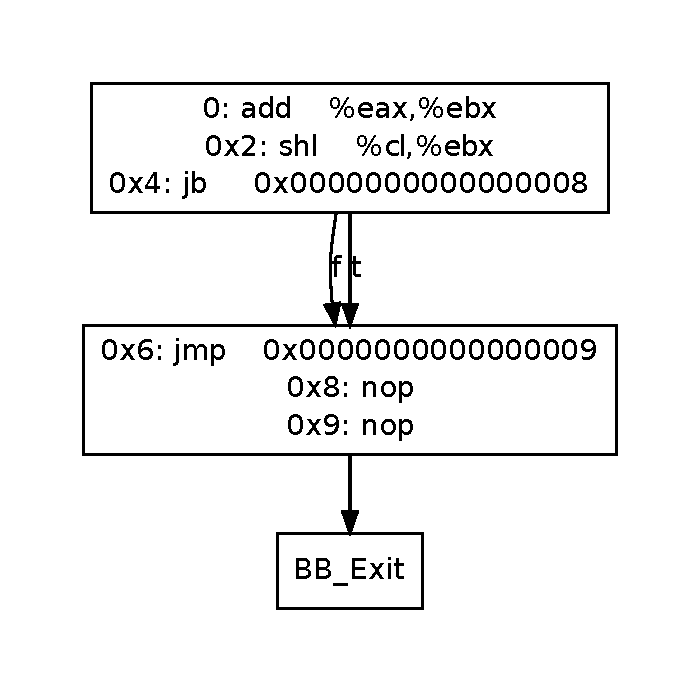
\includegraphics[height=3in]{chap-examples/cfg2.pdf}
  \end{center}
  \caption{Example Basic CFG}
  \label{fig:basiccfg}
\end{figure}

\begin{figure}[!p]
  \begin{center}
    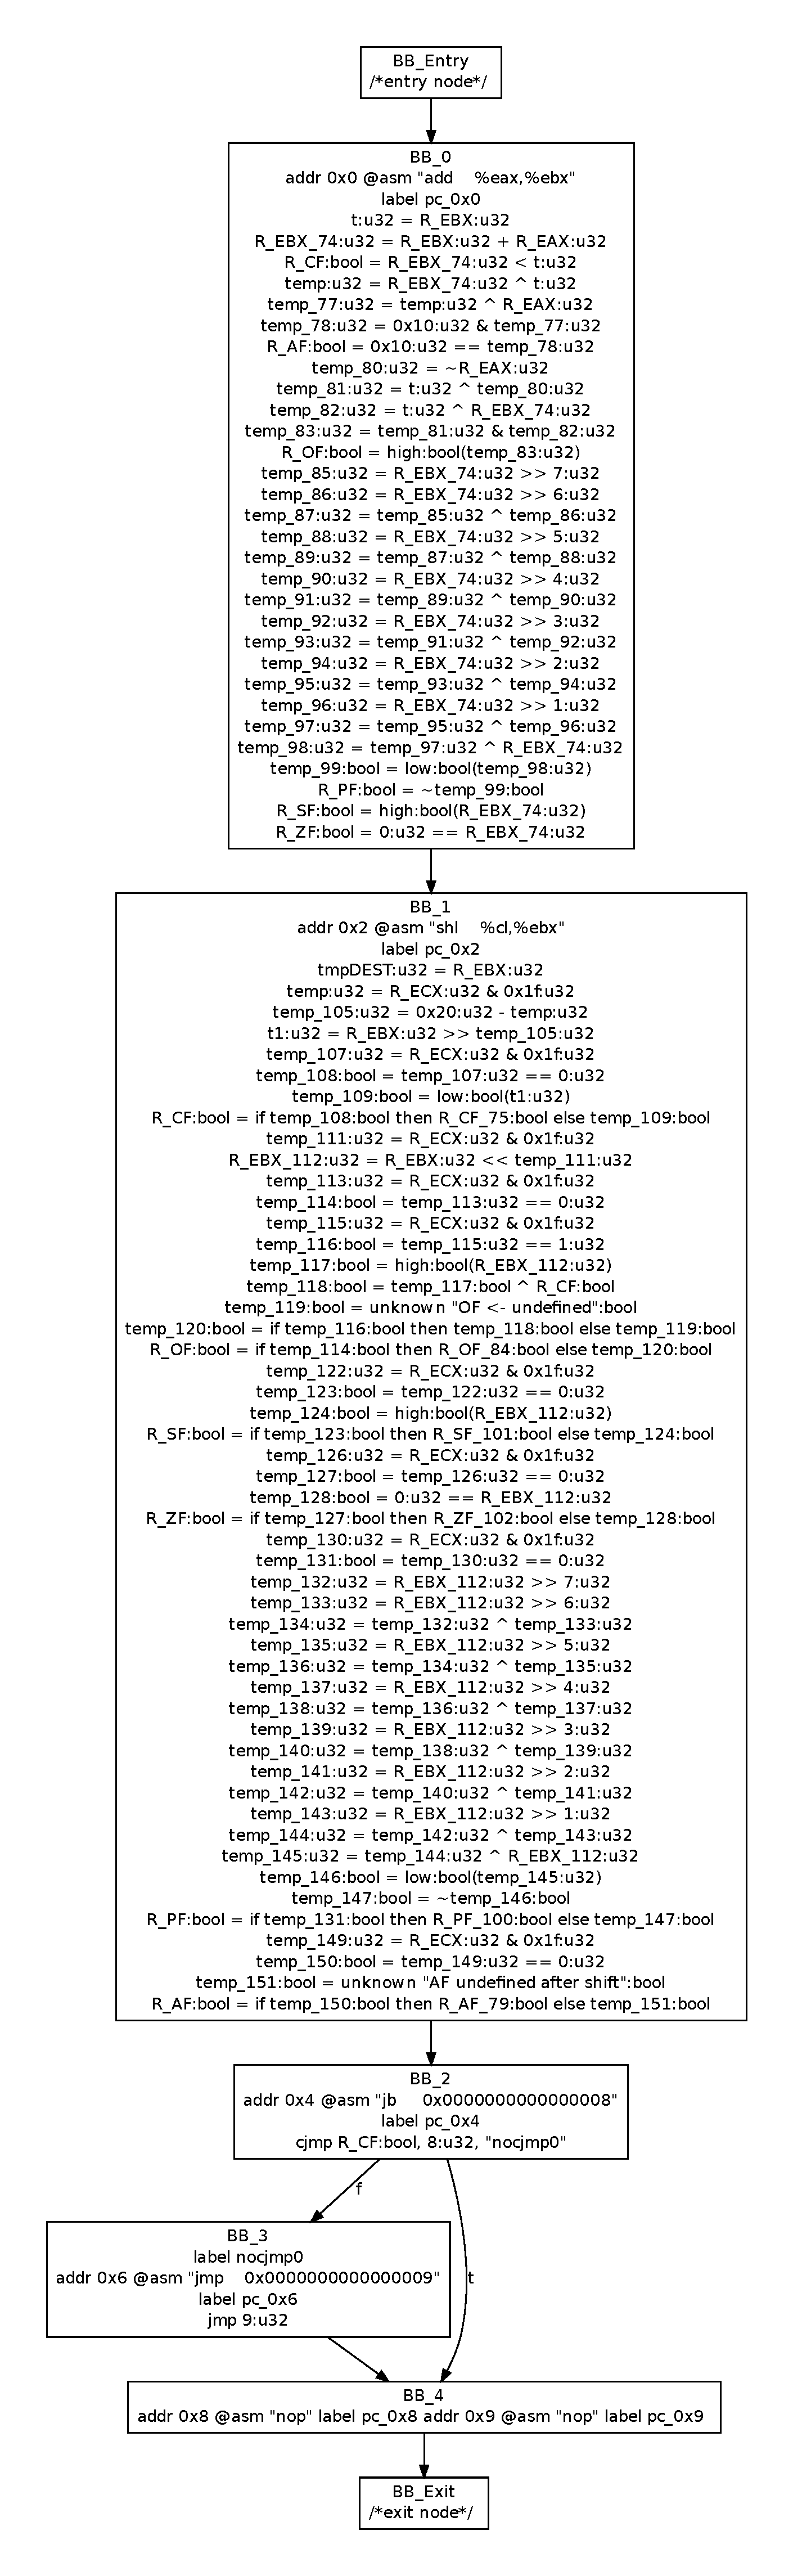
\includegraphics[height=.9\textheight]{chap-examples/cfg.pdf}
  \end{center}
  \caption{Example Detailed CFG}
  \label{fig:cfg}
\end{figure}

\begin{figure}[p]
  \begin{center}
    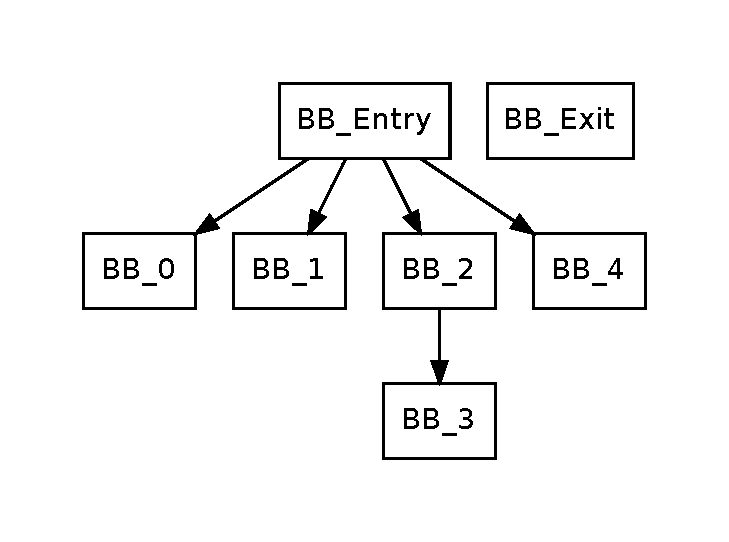
\includegraphics{chap-examples/cdg.pdf}
  \end{center}
  \caption{Example CDG}
  \label{fig:cdg}
\end{figure}

\begin{figure}[p]
  \begin{center}
    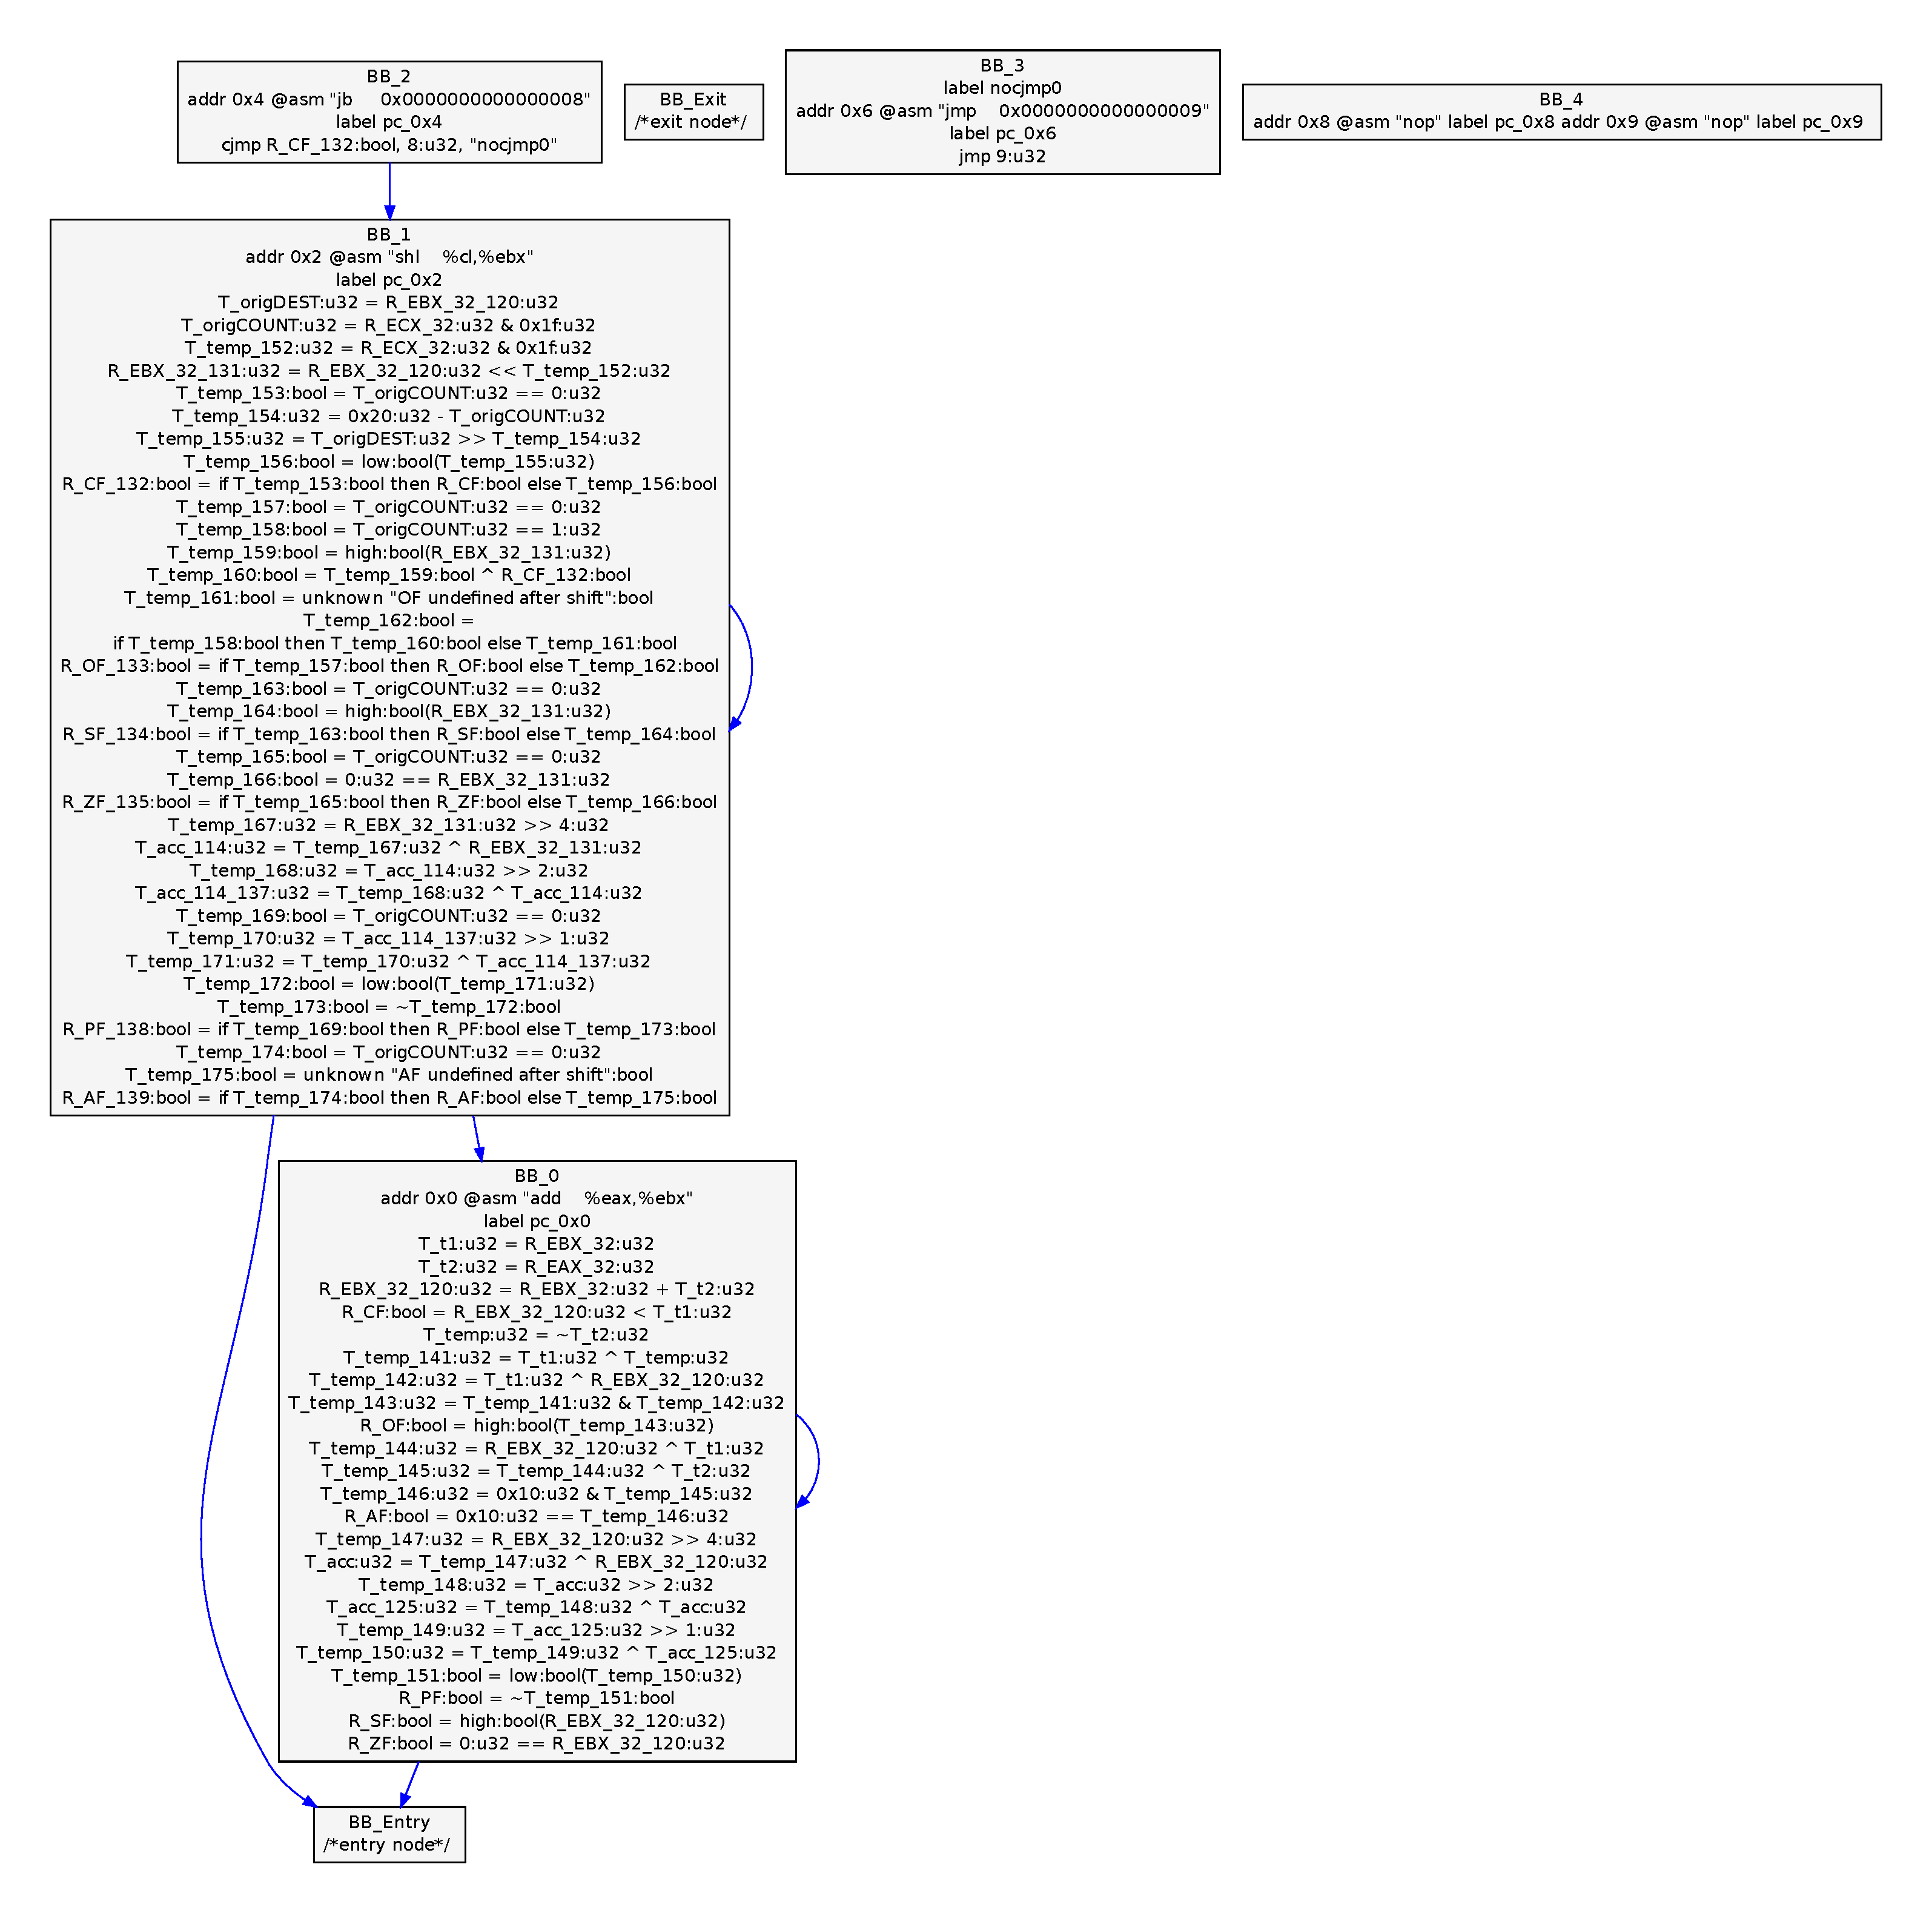
\includegraphics[height=.9\textheight]{chap-examples/ddg.pdf}
  \end{center}
  \caption{Example DDG}
  \label{fig:ddg}
\end{figure}

\begin{figure}[p]
  \begin{center}
    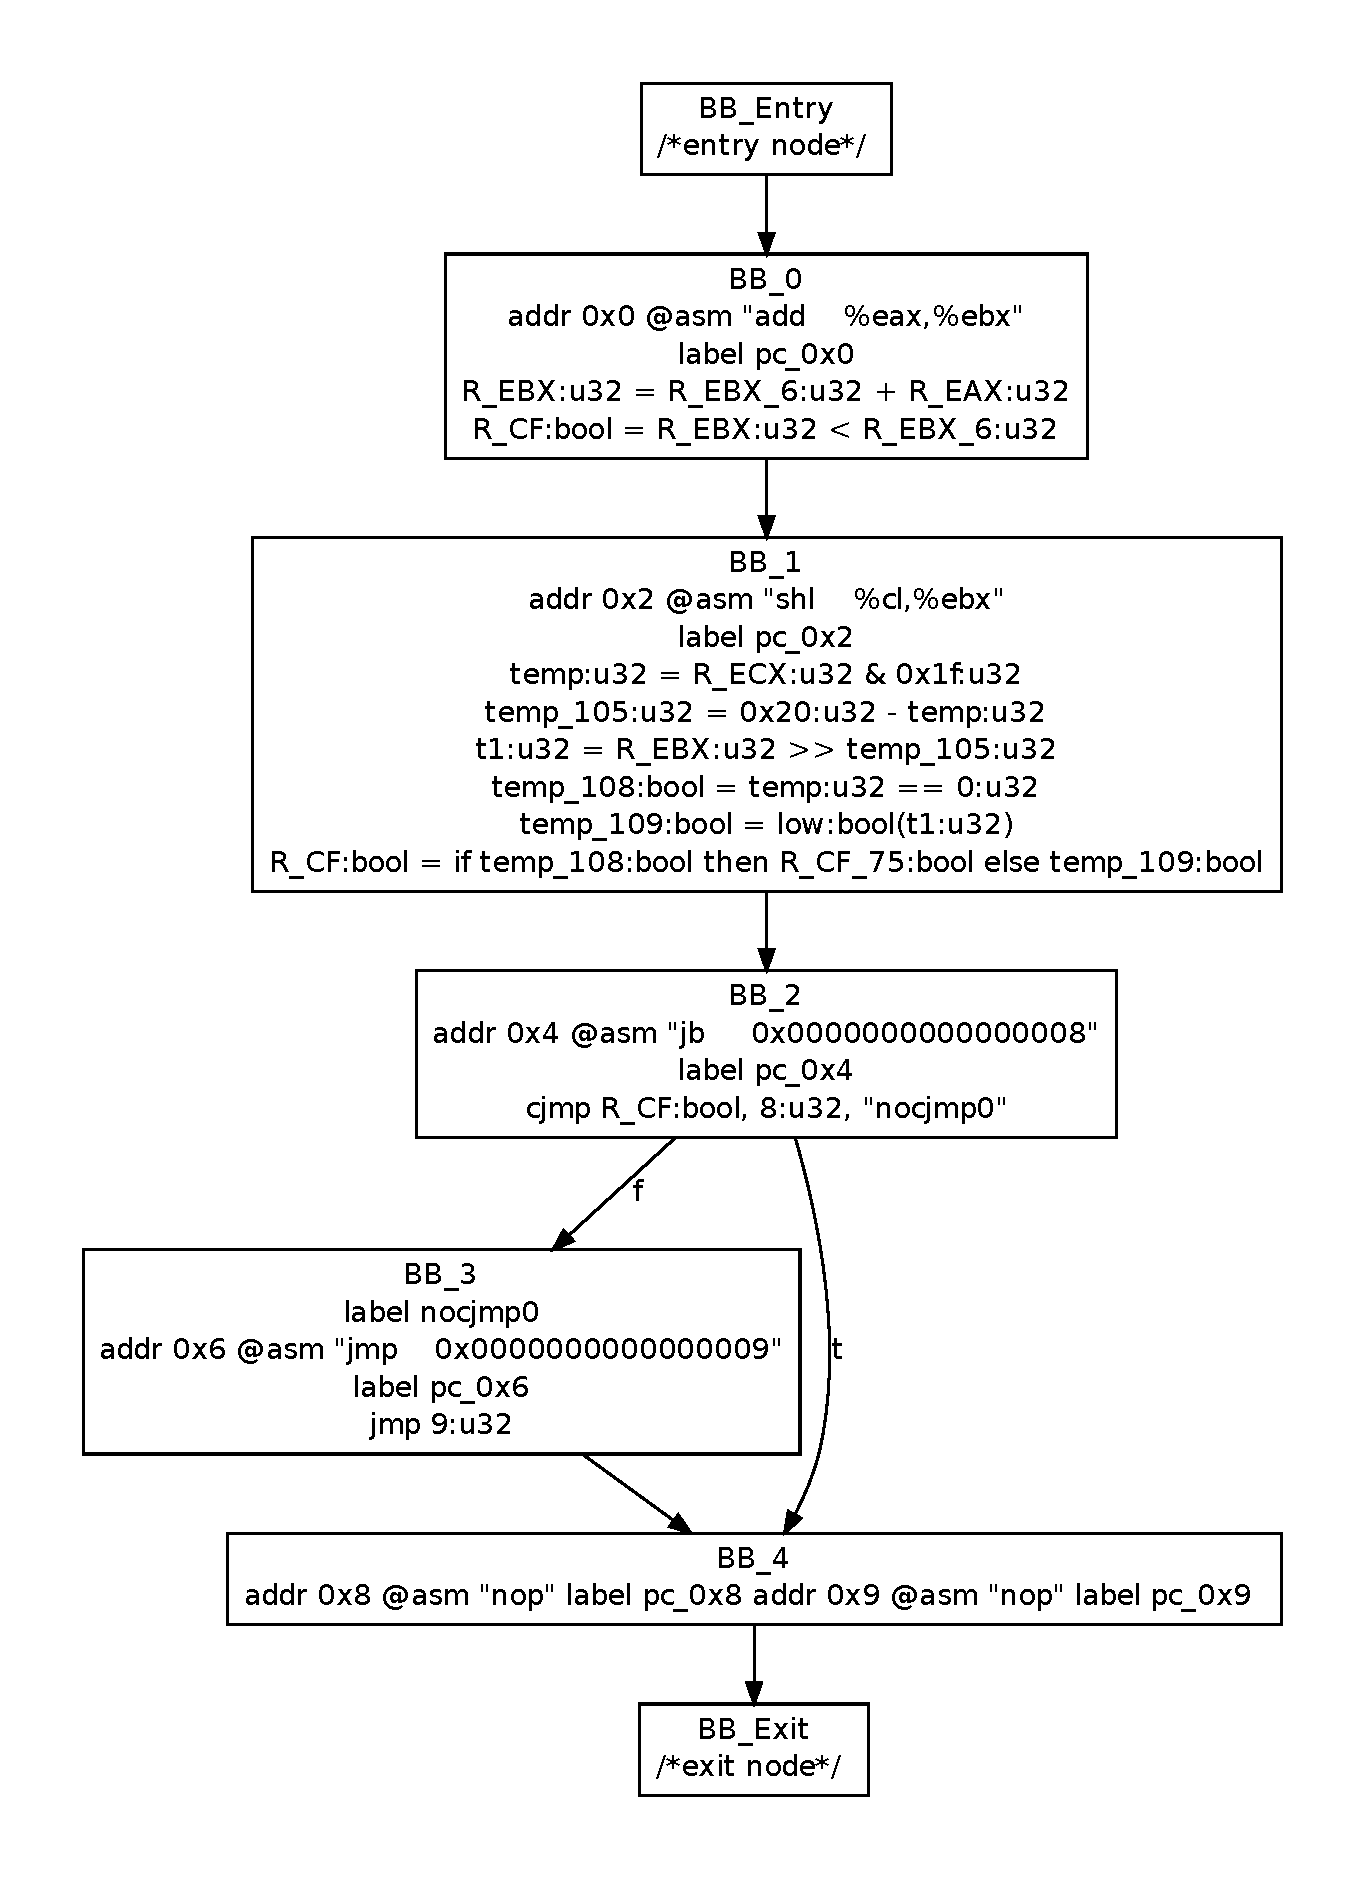
\includegraphics[height=.9\textheight]{chap-examples/cfg_simp.pdf}
  \end{center}
  \caption{Example Simplified CFG}
  \label{fig:cfgsimp}
\end{figure}
\FloatBarrier

\subsection{Verification Conditions}

Let's say we want to know if we can take the jump at address four.  We
can test this in BAP by using verification conditions (VCs).  To do
this, we need to add a helper variable to the IL that represents
success.  We can do this by setting the goal variable to false at the
beginning of the program, and setting it to true after the branch is
taken.  Below is the modified IL that does this.

\verbatiminput{chap-examples/basic_mod.il}

To see if we take the jump, we can use topredicate with the post
condition \cmdline{goal}: \cmdline{topredicate -q -il basic\_mod.il
  -stp-out /tmp/f -post goal -solve}.  This will create a VC, and then
solve it using the \cmdline{stp} solver.  \cmdline{stp} returned
\begin{verbatim}
R_ECX_7 -> 0x3
R_EAX_5 -> 0x20000000
R_EBX_6 -> 0
\end{verbatim}
as a satisfying answer. Sure enough, $0x0 + 0x20000000 = 0x20000000$
and $0x20000000 << 0x3$ sets the carry flag, so the program would take the jump.

%%% Local Variables: 
%%% mode: latex
%%% TeX-master: "../main"
%%% End: 

\section{Concrete Evaluation}

In this tutorial, we will explain how to raise a binary to the BAP IL,
and then evaluate the resulting code inside of BAP.

Let's start with the following simple C program:
\verbatiminput{chap-examples/test.c}

We can compile this source file (named test.c) to a binary using
\cmdline{gcc -static test.c -o test} (note if you are on an x64 machine you may
need to add the \cmdline{-m32} option).  We use the \cmdline{-static} option of
gcc here because the BAP evaluator needs to know what code is located
at each memory location. This means that BAP does not currently
support self-modifying code, or dynamic linking (unless the user
explicitly tells BAP the mapping of memory addresses to binary code).

Once we have a binary, we can then raise it to the BAP IL by executing
\cmdline{toil -bin test -o test.il}. We can now disassemble the binary
to see where main begins and ends -- we will need this to tell BAP
where to start and stop executing. Here is a possible disassembly of
the main function.

\begin{verbatim}
08048267 <main>:
 8048267:       55                      push   %ebp
 8048268:       89 e5                   mov    %esp,%ebp
 804826a:       83 ec 04                sub    $0x4,%esp
 804826d:       c7 04 24 2a 00 00 00    movl   $0x2a,(%esp)
 8048274:       e8 d7 ff ff ff          call   8048250 <g>
 8048279:       c9                      leave  
 804827a:       c3                      ret    
 804827b:       90                      nop
 804827c:       90                      nop
 804827d:       90                      nop
 804827e:       90                      nop
 804827f:       90                      nop
\end{verbatim}

For this sample disassembly, we can begin execution at address
0x8048267.  Likewise, we can halt execution at 0x804827a.  To make BAP
halt execution, we'll manually add a halt command to the lifted IL.
For this example, you could search for the string
\verb!addr 0x804827a! in test.il, which marks the beginning of the ret
instruction in the lifted IL.  Inserting \verb!halt R_EAX:u32!  after
the address and label statements will cause the evaluator to halt and
return the value in eax.  For instance:

\begin{verbatim}
addr 0x804827a @asm "ret    "
label pc_0x804827a
halt R_EAX:u32
\end{verbatim}

Now, issue \cmdline{ileval -il test.il -eval-at mainaddr}, where
mainaddr is the address to start from.  BAP will evaluate the IL
program.  If debugging output is enabled (by setting the
\texttt{BAP\_DEBUG\_MODULES} environment variable to
\texttt{Symbeval}), it will print each statement as it is evaluated.
After halting, BAP will print the return value, which is
eax. Unsurprisingly, the returned value of eax is 42.

Now let's begin execution starting from the call instruction in main
(0x8048250). This will allow us to modify the input to the function
g. The -init-var and -init-mem options allow the user to specify an
initial value for a variable (register) or memory address
respectively.  To replicate what we just did and use an input of 42,
we can use the following the command \cmdline{ileval -il test.il
  -init-mem R\_ESP:u32 42:u32 -eval-at 0x8048274}. Notice that this
begins execution at the call instruction instead of the beginning of
main.  Unsurprisingly, eax has a final value of 42 again.  If we
instead change the memory pointed to by esp to 43, by \cmdline{ileval
  -il test.il -init-mem R\_ESP:u32 43:u32 -eval-at 0x8048274}, eax has
a final value of -1.

\section{Traces}

In this section, we will explain how to use our PIN-based trace
recording tool to record a trace.  We then show how to perform common
trace analysis tasks.

\subsection{Setup}

The PIN trace tool is located in the \cmdline{pintraces/}
directory.  Because of licensing reasons, we cannot distribute PIN
with the trace tool.  PIN must be extracted inside of the traces
directory; for instance, if the traces branch is located in
\cmdline{\$PATH/traces}, then PIN should be in
\cmdline{\$PATH/traces/pin}.  Running ./getpin.sh from the
\cmdline{\$PATH/traces/pintraces} directory will automatically
download and install PIN for Linux; the user is responsible for
accepting the PIN license agreements.  On Windows, PIN must be
downloaded and extracted by hand.  The PIN tool can be built by
executing \cmdline{make} in the \cmdline{\$PATH/traces/experiemental}
directory.  On Windows, we reccomend using GNU Make for Windows
(\url{http://gnuwin32.sourceforge.net/packages/make.htm}) and Visual
C++ 2010 express
(\url{http://www.microsoft.com/visualstudio/en-us/products/2010-editions/visual-cpp-express}).
After compilation, the PIN tool should exist in \\
\cmdline{\$PATH/traces/pintraces/obj-ia32/gentrace.so} (or
gentrace.dll on Windows).  In the rest of the chapter, we will assume
Linux is being used; most interaction with the trace tool is the same.

\subsection{Recording a trace}

To see the command line options to the trace tool, execute 

\begin{verbatim} 
$PATH/traces/pin/pin -t
$PATH/traces/pintraces/obj-ia32/gentrace.so -h -- /bin/ls
\end{verbatim}.

By default, the trace tool will only log instructions that are
\emph{tainted}, i.e., those that depend on user input.  The options
that begin with taint are used to mark various data
as being user input.  For instance, -taint-files readme marks the file
readme as being user input.

We will record a trace of a simple buffer overflow.  Run 

\begin{verbatim}
echo ``helloooooooooooooooooo'' > readme
\end{verbatim}

 to create the input file.  Then run 

\begin{verbatim}
$PATH/traces/pin/pin -t 
$PATH/traces/pintraces/obj-ia32/gentrace.so -taint-files readme
$PATH/traces/pintraces/examples/bof
\end{verbatim}

The PIN tool will output
many debugging messages; this is normal.  If the trace tool detected
the buffer overflow, it will print ``stack smashing detected'' near
the end of the logs.  At this point, there should be a trace file
ending with suffix bpt in the current working directory.  In the
following commands, we assume this file is named trace.bpt.

To lift the trace data and print it, run 

\begin{verbatim}
iltrans -pin -trace trace.bpt -pp-ast /dev/stdout
\end{verbatim}

It is also possible to concretize the trace, which removes jumps and performs
memory concretization, by executing 

\begin{verbatim}
iltrans -pin -trace trace.bpt -trace-concrete -pp-ast /dev/stdout
\end{verbatim}

Adding the -trace-check option before -trace-concrete causes BAP to compare its
internal evaluator's notion of state with the actual values recorded in the
trace.  It can be used to check for bugs in the IL.  Finally, running 

\begin{verbatim}
iltrans -pin -trace trace.bpt -trace-formula f
\end{verbatim}

will symbolically execute the trace and output the generated verification
condtion to the file f. This can then be solved with stp to find satisfying
answers to the trace.



%\section{Discussion}
\label{vine:discussion}

\subsection{Why Design a New Infrastructure?}  

At a high level, we designed \bap as a new platform because existing
platforms are a) defined for higher-level languages and thus not
appropriate for binary code analysis, b) designed for orthogonal goals
such as binary instrumentation or decompilation, and/or c) unavailable
to use for research purposes.  As a result, other tools we tried
(e.g., DynInst~\cite{dyninst} version 5.2, Phoenix~\cite{phoenix}
April 2008 SDK, IDA Pro~\cite{idapro} version 5, and others) were
inadequate, e.g., could not create a correct control flow graph for
the 3 line assembly shown in Figure~\ref{vine:shl-add}. Another reason
we created \bap is so that we could be sure of the semantics of 
analysis. Existing platforms tend not to have publicly available
formally defined semantics, thus we would not know exactly what we are
using.

Formal semantics are important for several practical reasons. We found
that defining the semantics of \bap was helpful in catching design
bugs, unsupported assumptions, and other errors that could affect many
different kinds of analysis. In addition, the semantics are helpful
for communicating how \bap works with other researchers.  Further,
without a specified semantics, it is difficult to show an analysis is
correct. For example, in ~\cite{brumley:2006:alias} we show our
proposed assembly-level alias analysis~\cite{brumley:2006:alias} is
correct with respect to the operational semantics of \bap.


\subsection{Limitations of \bap}

\begin{description}
\item[Architectures] \bap only supports x86 right now.  We intend to
  add support for x86-64 and ARM in the future.
\item[Semantics] \bap is designed to enable program analysis of binary
  program states. Therefore, analyses that depend upon more than the
  operational semantics of the instruction fall outside the scope of
  \bap. For example, creating an analysis of the timing behavior of
  binary programs falls outside the current scope of \bap.
\item[User-mode instructions] \bap only models user-mode level
  instructions.  Unhandled instructions will be lifted as {\tt
    special} statements or {\tt unknown} expressions.
\item[Integer instructions] \bap only models instructions that
  manipulate integers.  In particular, \bap does not model floating
  point instructions.
\item[Indirect jumps] \bap does not currently resolve indirect jumps,
  or perform ``CFG recovery''.  We plan to add this in a future
  release.
\end{description}

\subsection{Is Lifting Correct?}

Assembly instructions are lifted to \bap in a syntax directed manner.
One may view the \bap IL as a model of the underlying assembly.  There
is a chance, however, that lifting could produce incorrect
IL. Although it is impossible to say that all assembly instructions
are correctly lifted, the advantage of \bap's design is that only the
lifting process needs to understand the semantics of the original
assembly.

We perform nightly testing to make sure that \bap's model of execution
matches what happens on a real x86 processor.  Our nightly tests also
tell us which instructions are used in our test programs that are not
modeled in \bap.  The results of these tests are always available at
\url{http://bap.ece.cmu.edu/nightly-reports/}.

\subsection{Size of Lifting IL for a Program}

A single assembly instruction will typically be translated into
several \bap statements. Thus, the resulting \bap program will have
more statements than the corresponding assembly.  For example and
roughly speaking, x86 assembly instructions are raised to be about 7
\bap statements: 1 \bap statement for the direct effect, and 6 for
updating processor-specific status flags.

In our experience, the constant-size factor in code size is worth the
benefits of simplifying the semantics of assembly.  Assembly
instructions are designed to be efficient for a computer to execute,
not for a human to understand. The IL, on the other hand, is designed
to be easy for a human to understand.  We have found even experienced
assembly-level programmers will comment that they have a hard time
keeping track of control and data dependencies since there are few
syntactic cues in assembly to help. \bap, on the other hand, obviates
all data and control dependencies within the code. 

%%% Local Variables: 
%%% mode: latex
%%% TeX-master: "../main"
%%% End: 


\chapter{Related Work}
\label{vine:related}

\paragraph{Other Binary Analysis Platforms.} \bap is designed to 1)
have a formal, well-defined IL, 2) explicitly expose the semantics of
complex assembly in terms of the simpler \bap IL, and 3) be easy to
re-target.  There are several other binary analysis platforms which
may have some similarity to \bap, do not fulfill all requirements.

Phoenix is a program analysis environment developed by Microsoft as
part of their next generation compiler~\cite{phoenix}. One of the
Phoenix tools allows Microsoft compiled code to be raised up to a
register transfer language (RTL).  A RTL is a low-level IR that
resembles an architecture-neutral assembly.

Phoenix differs from \bap in several ways. First, Phoenix can only
lift code produced by a Microsoft compiler. Second, Phoenix requires
debugging information, thus is not a true binary-only analysis
platform.  Third, Phoenix lifts assembly to a low-level IR that does
not expose the semantics of complicated instructions, e.g., register
status flags, as part of the IR~\cite{phoenix:noflags}. Fourth, the
semantics of the lifted IR, as well as the lifting semantics and
goals, are not well specified~\cite{phoenix:noflags}, and thus not
suitable for our research purposes.


The CodeSurfer/x86 platform~\cite{balakrishnan:2005} is a proprietary
platform for analyzing x86 programs. At the core of CodeSurfer/x86 is a
value-set analysis (VSA)~\cite{balakrishnan:2007}.  We have also
implemented VSA in \bap.  CodeSurfer/x86 was not made available for
comparison, thus we do not know whether it supports a well-defined IL,
is re-targetable, or what other comparable aspects it may share with \bap.

\paragraph{Decompilation.} Decompilation is the process of inverting
the compilation of a program back to the original source
language. Generally, the goal of decompilation is to recover a valid
program in the original source language that is semantically
equivalent (though need not be exactly the same) as the original
source program.  

Program analysis is often an important component in the decompilation
process. Cifuentes has proposed using data and control flow analyses
as part of decompilation~\cite{cifuentes:1994}.  Van Emmerik has shown
that analysis on SSA flow graphs is helpful in a variety of tasks such
as reconstructing types and resolving indirect
jumps~\cite{vanemmerik:2007}.  \bap also has SSA;  thus it should
be straight-forward to implement Van Emmerik's algorithms. Mycroft has
proposed type inference for recovering C types during
decompilation~\cite{mycroft:1999}.  Adding type inference is a
possible future direction for \bap.


\paragraph{Binary Instrumentation.} Binary instrumentation is a
technique to insert extra code into a binary that monitors the
instrumented program's behavior
(e.g.,~\cite{srivastava:1994,larus:1995,luk:2005,nethercote:2004:phd,nanda:2006,dynamorio,dyninst}). Instrumentation
is performed by inserting jumps in the original binary code to the
instrumentation code.  The instrumentation code then jumps back to the
original code after executing. The instrumentation code must make sure
that the execution state is the same before and after the jump in
order for the instrumentation to be transparent.

Although many binary instrumentation tools provide a limited amount of
program analysis, the end-goal is instrumentation, not facilitating
analyses.  For example, Pin~\cite{luk:2005} calculates register
liveness information. However, general static analysis is outside the
scope of such tools. For instance, instrumentation tools generally do
not expose the semantics of all instructions such as register status
flag updates.


\paragraph{Other Program Analysis Platforms.} \bap shares many of the same
goals, such as modularity and ease of writing correct analyses, as
other program analysis platforms.  For example,
CIL~\cite{necula:2002:cil} and SUIF~\cite{suif} are both excellent
platforms for analyzing C code.  However, using higher-level program
analysis platforms is inappropriate for binary code because binary
code is fundamentally different. While higher-level languages have
types, functions, pointers, loops, and local variables, assembly has
no types, no functions, one globally addressed memory region, and
goto's. The \bap IL and surrounding platform is designed specifically
to meet the challenges of faithfully analyzing assembly.




\chapter{Credits}
See \url{http://bap.ece.cmu.edu} for a list of current and former \bap
developers.



\bibliographystyle{plain}
\bibliography{bibtex/biblio,bibtex/misc}

\end{document}
